% Options for packages loaded elsewhere
\PassOptionsToPackage{unicode}{hyperref}
\PassOptionsToPackage{hyphens}{url}
%
\documentclass[
]{book}
\usepackage{amsmath,amssymb}
\usepackage{lmodern}
\usepackage{iftex}
\ifPDFTeX
  \usepackage[T1]{fontenc}
  \usepackage[utf8]{inputenc}
  \usepackage{textcomp} % provide euro and other symbols
\else % if luatex or xetex
  \usepackage{unicode-math}
  \defaultfontfeatures{Scale=MatchLowercase}
  \defaultfontfeatures[\rmfamily]{Ligatures=TeX,Scale=1}
\fi
% Use upquote if available, for straight quotes in verbatim environments
\IfFileExists{upquote.sty}{\usepackage{upquote}}{}
\IfFileExists{microtype.sty}{% use microtype if available
  \usepackage[]{microtype}
  \UseMicrotypeSet[protrusion]{basicmath} % disable protrusion for tt fonts
}{}
\makeatletter
\@ifundefined{KOMAClassName}{% if non-KOMA class
  \IfFileExists{parskip.sty}{%
    \usepackage{parskip}
  }{% else
    \setlength{\parindent}{0pt}
    \setlength{\parskip}{6pt plus 2pt minus 1pt}}
}{% if KOMA class
  \KOMAoptions{parskip=half}}
\makeatother
\usepackage{xcolor}
\usepackage{color}
\usepackage{fancyvrb}
\newcommand{\VerbBar}{|}
\newcommand{\VERB}{\Verb[commandchars=\\\{\}]}
\DefineVerbatimEnvironment{Highlighting}{Verbatim}{commandchars=\\\{\}}
% Add ',fontsize=\small' for more characters per line
\usepackage{framed}
\definecolor{shadecolor}{RGB}{248,248,248}
\newenvironment{Shaded}{\begin{snugshade}}{\end{snugshade}}
\newcommand{\AlertTok}[1]{\textcolor[rgb]{0.94,0.16,0.16}{#1}}
\newcommand{\AnnotationTok}[1]{\textcolor[rgb]{0.56,0.35,0.01}{\textbf{\textit{#1}}}}
\newcommand{\AttributeTok}[1]{\textcolor[rgb]{0.77,0.63,0.00}{#1}}
\newcommand{\BaseNTok}[1]{\textcolor[rgb]{0.00,0.00,0.81}{#1}}
\newcommand{\BuiltInTok}[1]{#1}
\newcommand{\CharTok}[1]{\textcolor[rgb]{0.31,0.60,0.02}{#1}}
\newcommand{\CommentTok}[1]{\textcolor[rgb]{0.56,0.35,0.01}{\textit{#1}}}
\newcommand{\CommentVarTok}[1]{\textcolor[rgb]{0.56,0.35,0.01}{\textbf{\textit{#1}}}}
\newcommand{\ConstantTok}[1]{\textcolor[rgb]{0.00,0.00,0.00}{#1}}
\newcommand{\ControlFlowTok}[1]{\textcolor[rgb]{0.13,0.29,0.53}{\textbf{#1}}}
\newcommand{\DataTypeTok}[1]{\textcolor[rgb]{0.13,0.29,0.53}{#1}}
\newcommand{\DecValTok}[1]{\textcolor[rgb]{0.00,0.00,0.81}{#1}}
\newcommand{\DocumentationTok}[1]{\textcolor[rgb]{0.56,0.35,0.01}{\textbf{\textit{#1}}}}
\newcommand{\ErrorTok}[1]{\textcolor[rgb]{0.64,0.00,0.00}{\textbf{#1}}}
\newcommand{\ExtensionTok}[1]{#1}
\newcommand{\FloatTok}[1]{\textcolor[rgb]{0.00,0.00,0.81}{#1}}
\newcommand{\FunctionTok}[1]{\textcolor[rgb]{0.00,0.00,0.00}{#1}}
\newcommand{\ImportTok}[1]{#1}
\newcommand{\InformationTok}[1]{\textcolor[rgb]{0.56,0.35,0.01}{\textbf{\textit{#1}}}}
\newcommand{\KeywordTok}[1]{\textcolor[rgb]{0.13,0.29,0.53}{\textbf{#1}}}
\newcommand{\NormalTok}[1]{#1}
\newcommand{\OperatorTok}[1]{\textcolor[rgb]{0.81,0.36,0.00}{\textbf{#1}}}
\newcommand{\OtherTok}[1]{\textcolor[rgb]{0.56,0.35,0.01}{#1}}
\newcommand{\PreprocessorTok}[1]{\textcolor[rgb]{0.56,0.35,0.01}{\textit{#1}}}
\newcommand{\RegionMarkerTok}[1]{#1}
\newcommand{\SpecialCharTok}[1]{\textcolor[rgb]{0.00,0.00,0.00}{#1}}
\newcommand{\SpecialStringTok}[1]{\textcolor[rgb]{0.31,0.60,0.02}{#1}}
\newcommand{\StringTok}[1]{\textcolor[rgb]{0.31,0.60,0.02}{#1}}
\newcommand{\VariableTok}[1]{\textcolor[rgb]{0.00,0.00,0.00}{#1}}
\newcommand{\VerbatimStringTok}[1]{\textcolor[rgb]{0.31,0.60,0.02}{#1}}
\newcommand{\WarningTok}[1]{\textcolor[rgb]{0.56,0.35,0.01}{\textbf{\textit{#1}}}}
\usepackage{longtable,booktabs,array}
\usepackage{calc} % for calculating minipage widths
% Correct order of tables after \paragraph or \subparagraph
\usepackage{etoolbox}
\makeatletter
\patchcmd\longtable{\par}{\if@noskipsec\mbox{}\fi\par}{}{}
\makeatother
% Allow footnotes in longtable head/foot
\IfFileExists{footnotehyper.sty}{\usepackage{footnotehyper}}{\usepackage{footnote}}
\makesavenoteenv{longtable}
\usepackage{graphicx}
\makeatletter
\def\maxwidth{\ifdim\Gin@nat@width>\linewidth\linewidth\else\Gin@nat@width\fi}
\def\maxheight{\ifdim\Gin@nat@height>\textheight\textheight\else\Gin@nat@height\fi}
\makeatother
% Scale images if necessary, so that they will not overflow the page
% margins by default, and it is still possible to overwrite the defaults
% using explicit options in \includegraphics[width, height, ...]{}
\setkeys{Gin}{width=\maxwidth,height=\maxheight,keepaspectratio}
% Set default figure placement to htbp
\makeatletter
\def\fps@figure{htbp}
\makeatother
\setlength{\emergencystretch}{3em} % prevent overfull lines
\providecommand{\tightlist}{%
  \setlength{\itemsep}{0pt}\setlength{\parskip}{0pt}}
\setcounter{secnumdepth}{5}
\newlength{\cslhangindent}
\setlength{\cslhangindent}{1.5em}
\newlength{\csllabelwidth}
\setlength{\csllabelwidth}{3em}
\newlength{\cslentryspacingunit} % times entry-spacing
\setlength{\cslentryspacingunit}{\parskip}
\newenvironment{CSLReferences}[2] % #1 hanging-ident, #2 entry spacing
 {% don't indent paragraphs
  \setlength{\parindent}{0pt}
  % turn on hanging indent if param 1 is 1
  \ifodd #1
  \let\oldpar\par
  \def\par{\hangindent=\cslhangindent\oldpar}
  \fi
  % set entry spacing
  \setlength{\parskip}{#2\cslentryspacingunit}
 }%
 {}
\usepackage{calc}
\newcommand{\CSLBlock}[1]{#1\hfill\break}
\newcommand{\CSLLeftMargin}[1]{\parbox[t]{\csllabelwidth}{#1}}
\newcommand{\CSLRightInline}[1]{\parbox[t]{\linewidth - \csllabelwidth}{#1}\break}
\newcommand{\CSLIndent}[1]{\hspace{\cslhangindent}#1}
\ifLuaTeX
  \usepackage{selnolig}  % disable illegal ligatures
\fi
\IfFileExists{bookmark.sty}{\usepackage{bookmark}}{\usepackage{hyperref}}
\IfFileExists{xurl.sty}{\usepackage{xurl}}{} % add URL line breaks if available
\urlstyle{same} % disable monospaced font for URLs
\hypersetup{
  pdftitle={A Minimal Book Example},
  pdfauthor={Vincent Godard},
  hidelinks,
  pdfcreator={LaTeX via pandoc}}

\title{A Minimal Book Example}
\author{Vincent Godard}
\date{2022-10-06}

\begin{document}
\maketitle

{
\setcounter{tocdepth}{1}
\tableofcontents
}
\hypertarget{prerequisites}{%
\chapter{Prerequisites}\label{prerequisites}}

This html page is derived from an \href{http://rmarkdown.rstudio.com}{R Markdown} Notebook.
You can copy/paste the various lines of code into your own R script and run it in any R session.

These activities do not require any specific prior knowledge of R programming language.
The idea is for you to simply copy and paste the code in a script, run it, and change various parameters to observe and investigate the associated response.

In addition to the scripting-oriented activities below you can also experiment visually with a few interactive \href{https://shiny.rstudio.com}{Shiny} apps

\url{http://shinyproxy.osupytheas.fr}

Both are built on the dedicated \texttt{TCNtools} package :

\url{https://vincentgodard.github.io/TCNtools}

This package contain various functions to assist the interpretation of TCN concentration at the Earth Surface.

You can install the package directly on you system (instructions on package website), or alternatively launch a binder session where everything is installed and should run smoothly.
You can launch the binder by clicking on the icon below, and access an online RStudio session in your browser.

\href{https://mybinder.org/v2/gh/VincentGodard/TCNtools/main?urlpath=rstudio}{\includegraphics{https://camo.githubusercontent.com/581c077bdbc6ca6899c86d0acc6145ae85e9d80e6f805a1071793dbe48917982/68747470733a2f2f6d7962696e6465722e6f72672f62616467655f6c6f676f2e737667}}

The first thing we have to do, before calling any of these functions, is to load the \texttt{TCNtools} package.

\begin{Shaded}
\begin{Highlighting}[]
\FunctionTok{library}\NormalTok{(}\StringTok{"TCNtools"}\NormalTok{)}
\end{Highlighting}
\end{Shaded}

\hypertarget{introduction}{%
\chapter{Introduction}\label{introduction}}

\hypertarget{objectives-of-the-session}{%
\section{Objectives of the session}\label{objectives-of-the-session}}

We are going to cover two things during this session

\begin{itemize}
\tightlist
\item
  look into the calculation of scaling factors used for the computation of local production rates, and how they vary in space and time
\item
  make some simple calculations of TCN concentration build up at the Earth surface, as a response to exposure and denudation
\item
  test
\end{itemize}

\hypertarget{scaling-factors}{%
\chapter{Scaling factors}\label{scaling-factors}}

First we are going to explore how the scaling factors are changing with elevation, latitude and time, and what is the impact on local production rates.

\hypertarget{time-independent-scaling}{%
\section{Time-independent scaling}\label{time-independent-scaling}}

We are going to present the most widely used and simplest scaling scheme known as Lal-Stone and often abbreviated as \textbf{st}. The main equations are presented in the reference article by Stone (\protect\hyperlink{ref-stone2000air}{2000}) .

\hypertarget{site-characteristics}{%
\subsection{Site characteristics}\label{site-characteristics}}

We first need to define some parameters concerning the site of interest :

\begin{itemize}
\tightlist
\item
  latitude \texttt{lat} in degrees
\item
  altitude \texttt{z} in meters (can be a vector or a scalar)
\item
  longitude \texttt{lon} in degrees, this is not used for \emph{st} scaling (Stone (\protect\hyperlink{ref-stone2000air}{2000})), just in case we want to compute atmospheric pressure according to ERA40 (Uppala et al. (\protect\hyperlink{ref-uppala2005era40}{2005})).
\end{itemize}

\begin{Shaded}
\begin{Highlighting}[]
\NormalTok{lat }\OtherTok{=} \DecValTok{30} \CommentTok{\# latitude}
\NormalTok{lon }\OtherTok{=} \DecValTok{30} \CommentTok{\# longitude}
\NormalTok{z }\OtherTok{=} \FunctionTok{seq}\NormalTok{(}\DecValTok{0}\NormalTok{,}\DecValTok{3000}\NormalTok{,}\AttributeTok{by=}\DecValTok{100}\NormalTok{) }\CommentTok{\# vector from 0 to 3000 m by 100 m increments}
\end{Highlighting}
\end{Shaded}

Now we can compute the atmospheric pressure, with the function \texttt{atm\_pressure} according to the two models available, and then plot for comparison.
Here \texttt{z} is a vector to see the variations over a range of elevations.

To get information about the usage of the function used here (for example what are the different models) type \texttt{?atm\_pressure} in the R console.

\begin{Shaded}
\begin{Highlighting}[]
\NormalTok{P1 }\OtherTok{=} \FunctionTok{atm\_pressure}\NormalTok{(}\AttributeTok{alt=}\NormalTok{z,}\AttributeTok{model=}\StringTok{"stone2000"}\NormalTok{) }
\NormalTok{P2 }\OtherTok{=} \FunctionTok{atm\_pressure}\NormalTok{(}\AttributeTok{alt=}\NormalTok{z,}\AttributeTok{lat=}\NormalTok{lat,}\AttributeTok{lon=}\NormalTok{lon,}\AttributeTok{model=}\StringTok{"era40"}\NormalTok{)}
\FunctionTok{plot}\NormalTok{(P1,z,}\AttributeTok{type=}\StringTok{"l"}\NormalTok{,}\AttributeTok{xlab=}\StringTok{"Pressure (hPa)"}\NormalTok{,}\AttributeTok{ylab=}\StringTok{"Altitude (m)"}\NormalTok{,}\AttributeTok{col=}\StringTok{"darkorange3"}\NormalTok{) }
\FunctionTok{lines}\NormalTok{(P2,z,}\AttributeTok{lty=}\DecValTok{2}\NormalTok{,}\AttributeTok{col=}\StringTok{"darkorange3"}\NormalTok{)}
\FunctionTok{legend}\NormalTok{(}\StringTok{"topright"}\NormalTok{,}\FunctionTok{c}\NormalTok{(}\StringTok{"Stone 2000"}\NormalTok{,}\StringTok{"ERA40"}\NormalTok{),}\AttributeTok{lty=}\FunctionTok{c}\NormalTok{(}\DecValTok{1}\NormalTok{,}\DecValTok{2}\NormalTok{))}
\end{Highlighting}
\end{Shaded}

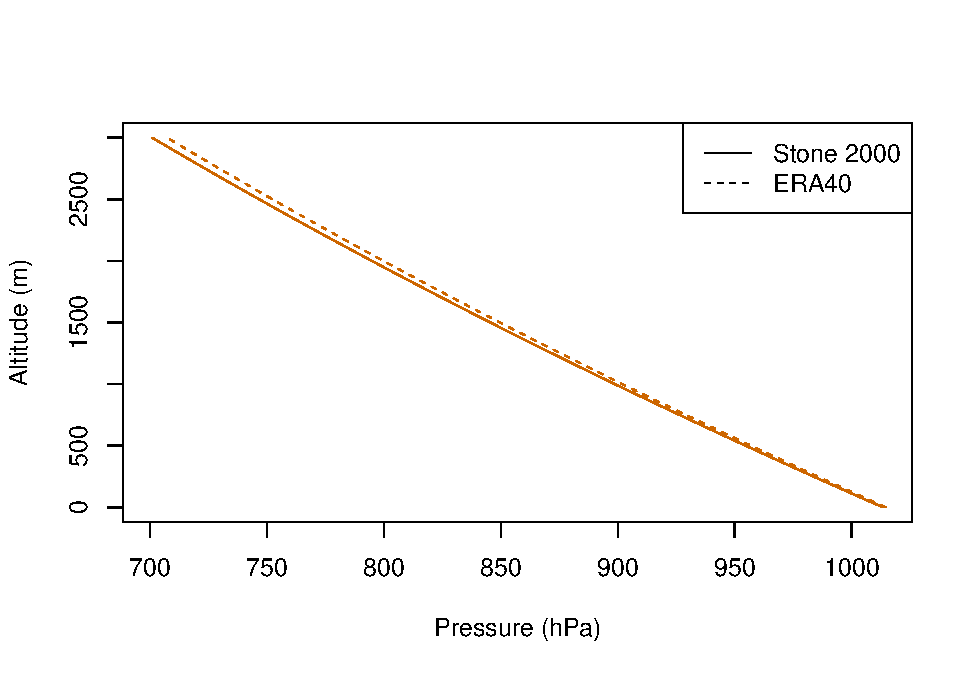
\includegraphics{_main_files/figure-latex/unnamed-chunk-4-1.pdf}

\begin{quote}
\textbf{TODO} Modify \texttt{lat} and \texttt{lon} to see the effects on the pressure computed with the ERA40 model
\end{quote}

\hypertarget{computation-of-scaling-factors}{%
\subsection{Computation of scaling factors}\label{computation-of-scaling-factors}}

We can now compute the scaling factors according to Stone (\protect\hyperlink{ref-stone2000air}{2000}).
Same as above, to get some information about the function (parameters definition) type \texttt{?st\_scaling} in the R console.

\begin{Shaded}
\begin{Highlighting}[]
\NormalTok{st }\OtherTok{=} \FunctionTok{scaling\_st}\NormalTok{(P1,lat) }\CommentTok{\# here we use the pressure according to Stone 2000 model}
\FunctionTok{print}\NormalTok{(st)}
\end{Highlighting}
\end{Shaded}

\begin{verbatim}
##    Nneutrons    Nmuons
## 1  0.8300224 0.8330000
## 2  0.9026631 0.8751951
## 3  0.9789258 0.9190924
## 4  1.0593995 0.9647381
## 5  1.1446610 1.0121787
## 6  1.2352759 1.0614606
## 7  1.3317993 1.1126307
## 8  1.4347771 1.1657357
## 9  1.5447466 1.2208226
## 10 1.6622372 1.2779383
## 11 1.7877718 1.3371297
## 12 1.9218669 1.3984436
## 13 2.0650339 1.4619266
## 14 2.2177794 1.5276253
## 15 2.3806062 1.5955858
## 16 2.5540138 1.6658541
## 17 2.7384989 1.7384759
## 18 2.9345563 1.8134963
## 19 3.1426788 1.8909602
## 20 3.3633586 1.9709117
## 21 3.5970868 2.0533946
## 22 3.8443547 2.1384521
## 23 4.1056535 2.2261264
## 24 4.3814748 2.3164594
## 25 4.6723113 2.4094921
## 26 4.9786564 2.5052644
## 27 5.3010052 2.6038156
## 28 5.6398539 2.7051842
## 29 5.9957004 2.8094072
## 30 6.3690443 2.9165212
## 31 6.7603872 3.0265612
\end{verbatim}

The result is stored in \texttt{st} as a dataframe with as many rows as there are elements in the input pressure vector (\texttt{P1}) and two columns named \texttt{Nneutrons} and \texttt{Nmuons}, for the spallogenic and muogenic contributions, respectively.

We can plot the evolution with elevation, which illustrates the major influence of altitude of the sampling site in controlling the local production rate.

\begin{Shaded}
\begin{Highlighting}[]
\FunctionTok{plot}\NormalTok{(st}\SpecialCharTok{$}\NormalTok{Nneutrons,z,}\AttributeTok{type=}\StringTok{"l"}\NormalTok{,}
     \AttributeTok{xlab=}\StringTok{"Spallogenic st scaling factor (Stone 2000)"}\NormalTok{,}\AttributeTok{ylab=}\StringTok{"Altitude (m)"}\NormalTok{,}
     \AttributeTok{main=}\FunctionTok{paste}\NormalTok{(}\StringTok{"Latitude "}\NormalTok{,lat,}\StringTok{"°"}\NormalTok{,}\AttributeTok{sep=}\StringTok{""}\NormalTok{),}\AttributeTok{col=}\StringTok{"darkorange3"}\NormalTok{)}
\end{Highlighting}
\end{Shaded}

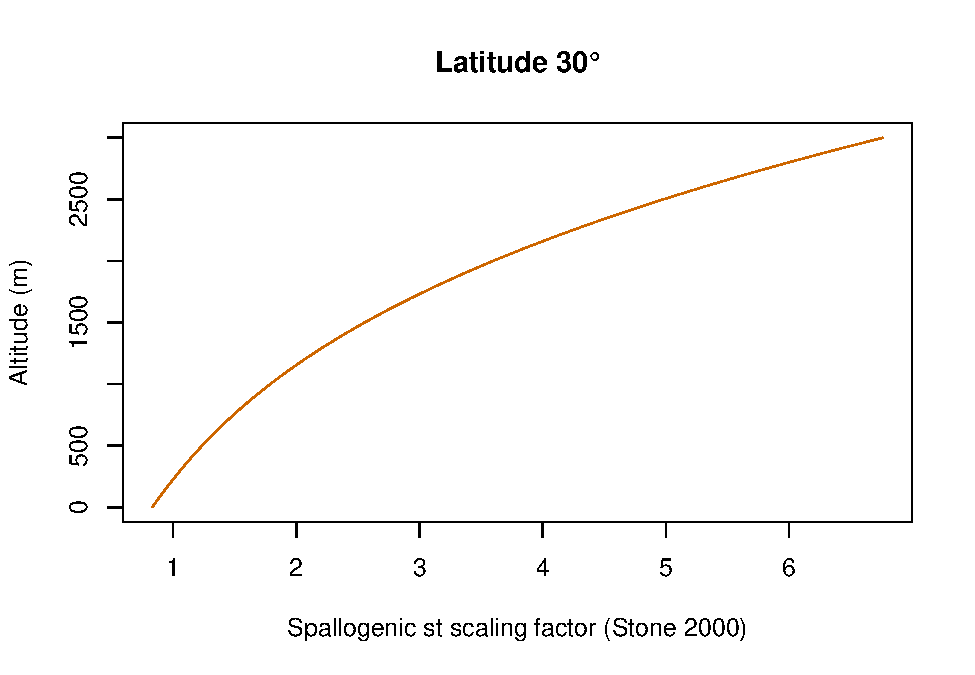
\includegraphics{_main_files/figure-latex/unnamed-chunk-6-1.pdf}

\begin{quote}
\textbf{TODO} Modify \texttt{lat} to see the effects on the scaling factor
\end{quote}

\hypertarget{global-variations}{%
\subsection{Global variations}\label{global-variations}}

In order to get a better idea of the variations with both latitude (from 0 to 90°) and elevation (from sea level to 3000 m) we can try the following plot.

\begin{Shaded}
\begin{Highlighting}[]
\NormalTok{P }\OtherTok{=} \FunctionTok{atm\_pressure}\NormalTok{(}\AttributeTok{alt=}\DecValTok{0}\NormalTok{,}\AttributeTok{model=}\StringTok{"stone2000"}\NormalTok{) }\CommentTok{\# compute pressure}
\NormalTok{lat }\OtherTok{=} \FunctionTok{seq}\NormalTok{(}\DecValTok{0}\NormalTok{,}\DecValTok{90}\NormalTok{,}\AttributeTok{by=}\DecValTok{1}\NormalTok{) }\CommentTok{\# latitude vector}
\NormalTok{n }\OtherTok{=} \FunctionTok{length}\NormalTok{(lat) }\CommentTok{\# size of vector}
\NormalTok{st }\OtherTok{=} \FunctionTok{scaling\_st}\NormalTok{(P,lat) }\CommentTok{\# compute scaling}
\FunctionTok{plot}\NormalTok{(lat,st}\SpecialCharTok{$}\NormalTok{Nneutrons,}\AttributeTok{type=}\StringTok{"l"}\NormalTok{,}\AttributeTok{ylim=}\FunctionTok{c}\NormalTok{(}\FloatTok{0.5}\NormalTok{,}\DecValTok{12}\NormalTok{),}\AttributeTok{col=}\StringTok{"darkorange3"}\NormalTok{,}
     \AttributeTok{xlab=}\StringTok{"Latitude (°)"}\NormalTok{,}\AttributeTok{ylab=}\StringTok{"Spallogenic st scaling factor (Stone 2000)"}\NormalTok{)}
\FunctionTok{grid}\NormalTok{()}
\FunctionTok{text}\NormalTok{(lat[n],st}\SpecialCharTok{$}\NormalTok{Nneutrons[n],}\StringTok{"0 km"}\NormalTok{,}\AttributeTok{cex=}\FloatTok{0.5}\NormalTok{,}\AttributeTok{adj=}\DecValTok{0}\NormalTok{) }\CommentTok{\# put label at the end of curve}
\ControlFlowTok{for}\NormalTok{ (z }\ControlFlowTok{in} \FunctionTok{seq}\NormalTok{(}\DecValTok{500}\NormalTok{,}\DecValTok{3000}\NormalTok{,}\AttributeTok{by=}\DecValTok{500}\NormalTok{))\{ }\CommentTok{\# loop on elevations : same as above for a range of elevations}
\NormalTok{  P }\OtherTok{=} \FunctionTok{atm\_pressure}\NormalTok{(}\AttributeTok{alt=}\NormalTok{z,}\AttributeTok{model=}\StringTok{"stone2000"}\NormalTok{) }
\NormalTok{  st }\OtherTok{=} \FunctionTok{scaling\_st}\NormalTok{(P,lat) }
  \FunctionTok{lines}\NormalTok{(lat,st}\SpecialCharTok{$}\NormalTok{Nneutrons,}\AttributeTok{col=}\StringTok{"darkorange3"}\NormalTok{)}
  \FunctionTok{text}\NormalTok{(lat[n],st}\SpecialCharTok{$}\NormalTok{Nneutrons[n],z}\SpecialCharTok{/}\DecValTok{1000}\NormalTok{,}\AttributeTok{cex=}\FloatTok{0.5}\NormalTok{,}\AttributeTok{adj=}\DecValTok{0}\NormalTok{)}
\NormalTok{\}}
\end{Highlighting}
\end{Shaded}

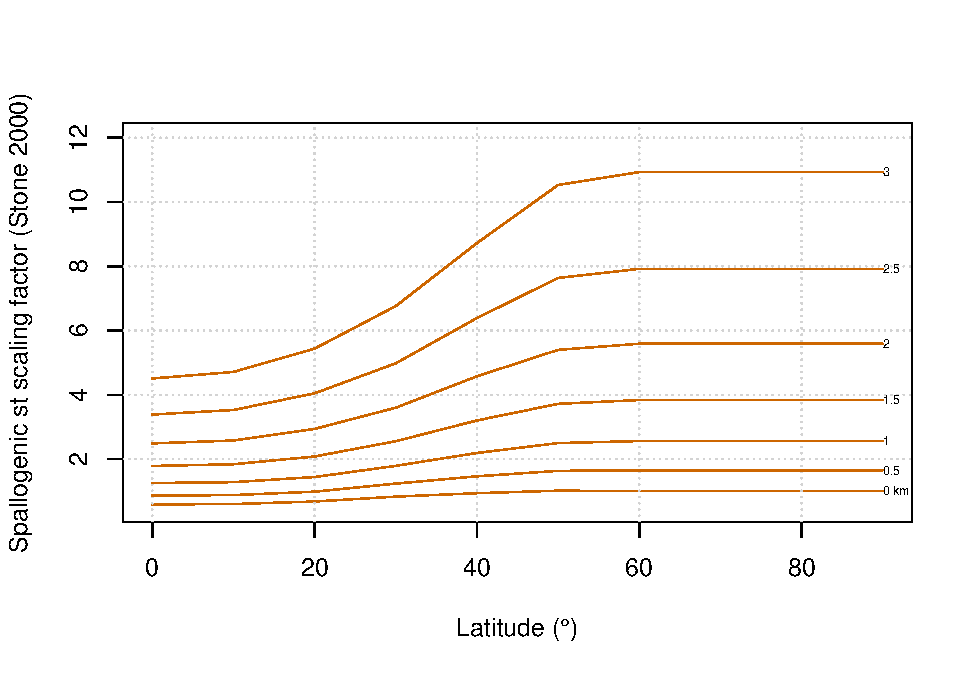
\includegraphics{_main_files/figure-latex/unnamed-chunk-7-1.pdf}

This dependence of the scaling factor on latitude is a direct consequence of the dipole structure of the Earth magnetic field, with a higher cosmic rays flux at high latitudes.

\hypertarget{time-dependent-scalings}{%
\section{Time-dependent scalings}\label{time-dependent-scalings}}

\hypertarget{definition-of-paleomagnetic-variations}{%
\subsection{Definition of paleomagnetic variations}\label{definition-of-paleomagnetic-variations}}

Time-dependent scaling factors allow to take into account the variations through time of the Earth magnetic field, which modulates the incoming cosmic ray flux. This is particularly important in exposure dating applications.

\hypertarget{virtual-dipole-moment}{%
\subsubsection{Virtual Dipole Moment}\label{virtual-dipole-moment}}

We need to first define a time series for the Virtual Dipole Moment (VDM) variation, using the \texttt{get\_vdm} function.

Several paleomagnetic database can be used.
The three options correspond to databases defined in \href{https://crep.otelo.univ-lorraine.fr}{Crep}.
We plot the three of them on the same graph.

\begin{Shaded}
\begin{Highlighting}[]
\NormalTok{time }\OtherTok{=} \FunctionTok{seq}\NormalTok{(}\DecValTok{0}\NormalTok{,}\FloatTok{50e3}\NormalTok{,}\AttributeTok{length.out =} \DecValTok{1000}\NormalTok{) }\CommentTok{\# time vector from 0 to 50 ka BP, with 1000 regularly spaced elements}
\CommentTok{\#}
\FunctionTok{plot}\NormalTok{(}\ConstantTok{NA}\NormalTok{,}\AttributeTok{xlim=}\FunctionTok{range}\NormalTok{(time),}\AttributeTok{ylim=}\FunctionTok{c}\NormalTok{(}\DecValTok{0}\NormalTok{,}\DecValTok{16}\NormalTok{),}\AttributeTok{xlab=}\StringTok{"Time (a BP)"}\NormalTok{,}\AttributeTok{ylab=}\StringTok{"VDM (10\^{}22 A.m\^{}2)"}\NormalTok{)}
\FunctionTok{grid}\NormalTok{()}
\CommentTok{\# {-} Glopis}
\NormalTok{col1}\OtherTok{=}\StringTok{"coral1"}
\NormalTok{vdm1}\OtherTok{=}\FunctionTok{get\_vdm}\NormalTok{(time,}\AttributeTok{model=}\StringTok{"glopis"}\NormalTok{)}
\FunctionTok{lines}\NormalTok{(time,vdm1}\SpecialCharTok{/}\FloatTok{1e22}\NormalTok{,}\AttributeTok{col=}\NormalTok{col1)}
\CommentTok{\# 2 {-} Musch}
\NormalTok{col2 }\OtherTok{=} \StringTok{"chartreuse"}
\NormalTok{vdm2}\OtherTok{=}\FunctionTok{get\_vdm}\NormalTok{(time,}\AttributeTok{model=}\StringTok{"musch"}\NormalTok{)}
\FunctionTok{lines}\NormalTok{(time,vdm2}\SpecialCharTok{/}\FloatTok{1e22}\NormalTok{,}\AttributeTok{col=}\NormalTok{col2)}
\CommentTok{\# 3 {-} lsd}
\NormalTok{col3 }\OtherTok{=} \StringTok{"cornflowerblue"}
\NormalTok{vdm3}\OtherTok{=}\FunctionTok{get\_vdm}\NormalTok{(time,}\AttributeTok{model=}\StringTok{"lsd"}\NormalTok{)}
\FunctionTok{lines}\NormalTok{(time,vdm3}\SpecialCharTok{/}\FloatTok{1e22}\NormalTok{,}\AttributeTok{col=}\NormalTok{col3)}
\FunctionTok{legend}\NormalTok{(}\StringTok{"topright"}\NormalTok{,}\FunctionTok{c}\NormalTok{(}\StringTok{"glopis"}\NormalTok{,}\StringTok{"musch"}\NormalTok{,}\StringTok{"lsd"}\NormalTok{),}\AttributeTok{col=}\FunctionTok{c}\NormalTok{(col1,col2,col3),}\AttributeTok{lty=}\DecValTok{1}\NormalTok{)}
\end{Highlighting}
\end{Shaded}

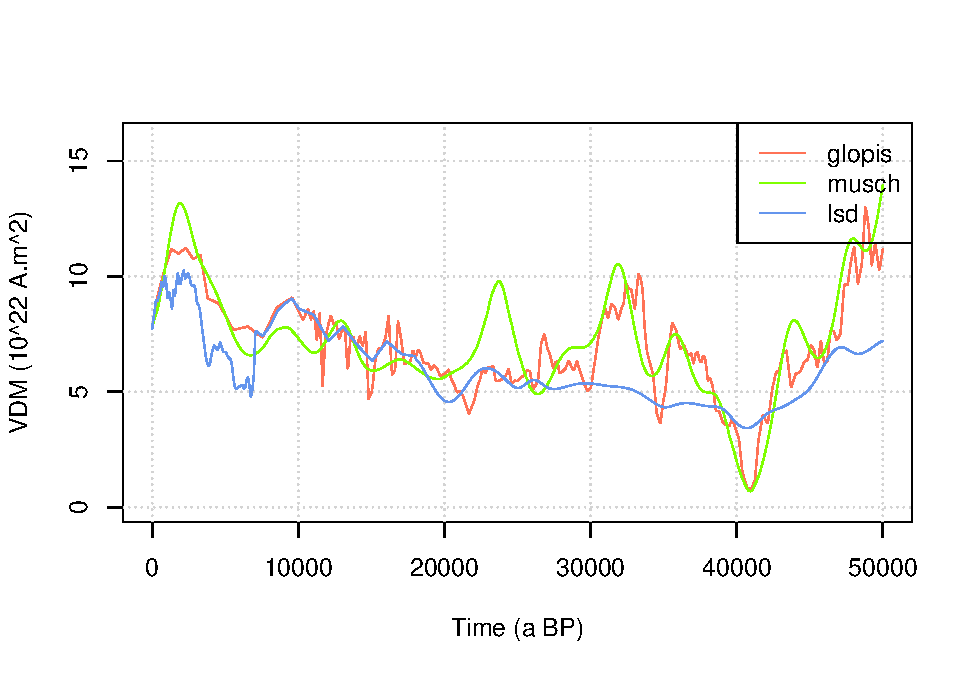
\includegraphics{_main_files/figure-latex/unnamed-chunk-8-1.pdf}

\hypertarget{cutoff-rigidity}{%
\subsubsection{Cutoff Rigidity}\label{cutoff-rigidity}}

Now we need to convert that into cutoff rigidity using \texttt{vdm2rc} function.
Such can be done using the following expression (Martin et al. (\protect\hyperlink{ref-martin2017crep}{2017})): \[R_c = 14.3 \frac{M}{M_0}\cos^4 \lambda,\] where \(M\) is the moment of the Earth dipole field, \(M_0\) the 2010 reference value for \(M\) and \(\lambda\) the latitude.
This corresponds to the default \texttt{model=elsasser54} in the \texttt{vdm2rc} function arguments.
A more complex formula proposed by Lifton, Sato, and Dunai (\protect\hyperlink{ref-lifton2014scaling}{2014}) can be used with \texttt{model=lifton14}.

\begin{Shaded}
\begin{Highlighting}[]
\NormalTok{lat }\OtherTok{=} \DecValTok{40}
\NormalTok{rc1a }\OtherTok{=} \FunctionTok{vdm2rc}\NormalTok{(vdm1,lat)}
\NormalTok{rc1b }\OtherTok{=} \FunctionTok{vdm2rc}\NormalTok{(vdm1,lat,}\AttributeTok{model=}\StringTok{"lifton14"}\NormalTok{)}
\NormalTok{rc2a }\OtherTok{=} \FunctionTok{vdm2rc}\NormalTok{(vdm2,lat)}
\NormalTok{rc2b }\OtherTok{=} \FunctionTok{vdm2rc}\NormalTok{(vdm2,lat,}\AttributeTok{model=}\StringTok{"lifton14"}\NormalTok{)}
\NormalTok{rc3a }\OtherTok{=} \FunctionTok{vdm2rc}\NormalTok{(vdm3,lat)}
\NormalTok{rc3b }\OtherTok{=} \FunctionTok{vdm2rc}\NormalTok{(vdm3,lat,}\AttributeTok{model=}\StringTok{"lifton14"}\NormalTok{)}
\CommentTok{\#}
\FunctionTok{plot}\NormalTok{(}\ConstantTok{NA}\NormalTok{,}\AttributeTok{xlim=}\FunctionTok{range}\NormalTok{(time),}\AttributeTok{ylim=}\FunctionTok{range}\NormalTok{(rc1a,rc2a,}\FunctionTok{na.omit}\NormalTok{(rc3a)),}\AttributeTok{xlab=}\StringTok{"Time (a BP)"}\NormalTok{,}\AttributeTok{ylab=}\StringTok{"Rc (GV)"}\NormalTok{)}
\FunctionTok{grid}\NormalTok{()}
\FunctionTok{lines}\NormalTok{(time,rc1a,}\AttributeTok{col=}\NormalTok{col1)}
\FunctionTok{lines}\NormalTok{(time,rc1b,}\AttributeTok{col=}\NormalTok{col1,}\AttributeTok{lty=}\DecValTok{2}\NormalTok{)}
\FunctionTok{lines}\NormalTok{(time,rc2a,}\AttributeTok{col=}\NormalTok{col2)}
\FunctionTok{lines}\NormalTok{(time,rc2b,}\AttributeTok{col=}\NormalTok{col2,}\AttributeTok{lty=}\DecValTok{2}\NormalTok{)}
\FunctionTok{lines}\NormalTok{(time,rc3a,}\AttributeTok{col=}\NormalTok{col3)}
\FunctionTok{lines}\NormalTok{(time,rc3b,}\AttributeTok{col=}\NormalTok{col3,}\AttributeTok{lty=}\DecValTok{2}\NormalTok{)}
\FunctionTok{legend}\NormalTok{(}\StringTok{"bottomleft"}\NormalTok{,}\FunctionTok{c}\NormalTok{(}\StringTok{"glopis"}\NormalTok{,}\StringTok{"musch"}\NormalTok{,}\StringTok{"lsd"}\NormalTok{,}\StringTok{"elsasser54"}\NormalTok{,}\StringTok{"lifton14"}\NormalTok{),}\AttributeTok{col=}\FunctionTok{c}\NormalTok{(col1,col2,col3,}\StringTok{"black"}\NormalTok{,}\StringTok{"black"}\NormalTok{),}\AttributeTok{lty=}\FunctionTok{c}\NormalTok{(}\DecValTok{1}\NormalTok{,}\DecValTok{1}\NormalTok{,}\DecValTok{1}\NormalTok{,}\DecValTok{1}\NormalTok{,}\DecValTok{2}\NormalTok{),}\AttributeTok{cex=}\FloatTok{0.5}\NormalTok{)}
\end{Highlighting}
\end{Shaded}

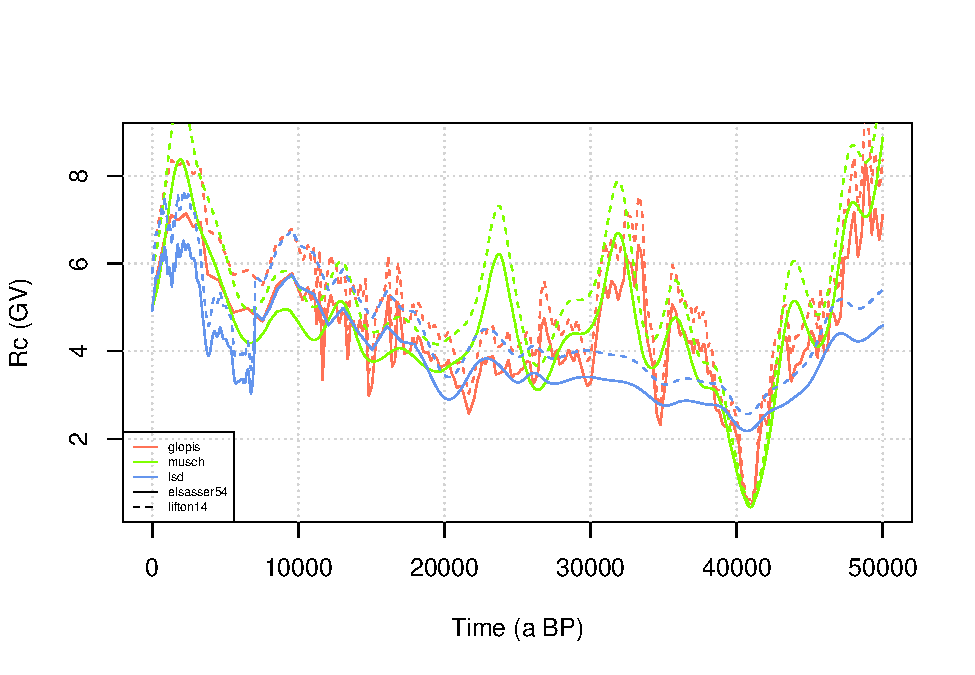
\includegraphics{_main_files/figure-latex/unnamed-chunk-9-1.pdf}

\begin{quote}
\textbf{TODO} change the latitude \texttt{lat} and observe the influence on \(R_c\)
\end{quote}

\hypertarget{lalstone-modified-scaling-lm}{%
\subsection{\texorpdfstring{Lal/Stone modified scaling (\emph{lm})}{Lal/Stone modified scaling (lm)}}\label{lalstone-modified-scaling-lm}}

Once we have a \(R_c\) time series we can compute the \emph{lm} scaling factors using the \texttt{scaling\_lm} function.
For that we will only use one elevation (\emph{z=0}), so we recompute the atmospheric pressure.
We plot the corresponding time series, as well as the value of \emph{st} scaling factor for reference.

\begin{Shaded}
\begin{Highlighting}[]
\NormalTok{P }\OtherTok{=} \FunctionTok{atm\_pressure}\NormalTok{(}\AttributeTok{alt=}\DecValTok{0}\NormalTok{,}\AttributeTok{model=}\StringTok{"stone2000"}\NormalTok{)}
\NormalTok{lm }\OtherTok{=} \FunctionTok{scaling\_lm}\NormalTok{(P,rc1a)}
\FunctionTok{plot}\NormalTok{(time,lm,}\AttributeTok{type=}\StringTok{"l"}\NormalTok{,}\AttributeTok{xlab=}\StringTok{"Time (a BP)"}\NormalTok{,}\AttributeTok{ylab=}\StringTok{"Spallogenic lm scaling factor"}\NormalTok{)}
\FunctionTok{abline}\NormalTok{(}\AttributeTok{h=}\FunctionTok{scaling\_st}\NormalTok{(P,lat)}\SpecialCharTok{$}\NormalTok{Nneutrons,}\AttributeTok{lty=}\DecValTok{2}\NormalTok{)}
\end{Highlighting}
\end{Shaded}

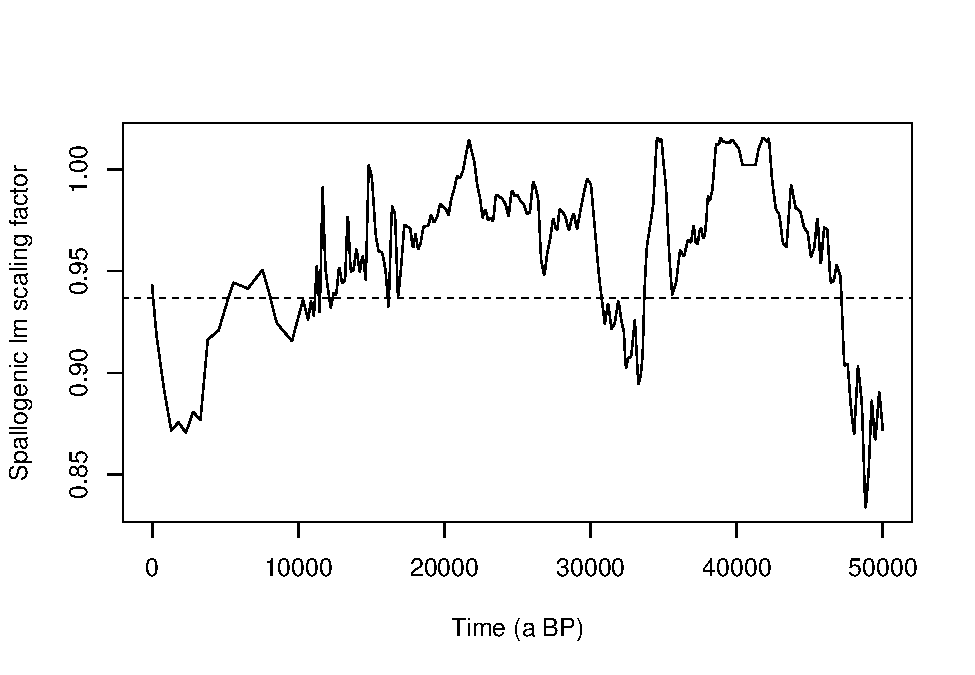
\includegraphics{_main_files/figure-latex/unnamed-chunk-10-1.pdf}

\begin{quote}
\textbf{TODO} Explore the variations of the scaling factor by using various values for elevation \texttt{alt}, and different \(R_c\) time-series. Look for the differences with the time-independant \texttt{st} scaling
\end{quote}

\hypertarget{interactive-app}{%
\section{Interactive App}\label{interactive-app}}

You can also explore dynamically the behavior of scaling parameters using this embedded application, which use the same type of code.

\hypertarget{exploring-tcn-build-up-at-the-surface}{%
\chapter{Exploring TCN build up at the surface}\label{exploring-tcn-build-up-at-the-surface}}

We are going to consider simple computations of concentration under various conditions in terms of erosion, depth or age.
This will be done using an \emph{Eulerian point of view}, which is the most straightforward and fastest way to perform such computation.
In this case the quantity of interest (concentration) is computed at fixed depths below the surface, while the exhumed material is moving through this reference frame during its trajectory toward the surface.
More details on the differences between Eulerian and Lagrangian approaches, and their applications to complex exposition/denudation histories, will be studied later.

Note that interpreting measured concentrations in terms of end-member situations of \emph{pure exposure} or \emph{steady-state denudation} is often done with online calculators (Balco et al. (\protect\hyperlink{ref-balco2008complete}{2008}),Marrero et al. (\protect\hyperlink{ref-marrero2016cronusearth}{2016}),Martin et al. (\protect\hyperlink{ref-martin2017crep}{2017})).
This will be fine in many cases, but you should always be careful about the underlying hypothesis (no erosion, steady state achieved\ldots) when interpreting your concentrations and always think about how TCN are accumulating.
The goal of this activity is to explore this behavior.

\hypertarget{background}{%
\section{Background}\label{background}}

The relevant general equation is the following,

\[
C=C_0e^{-\lambda t} + \sum_i \frac{P_i}{\frac{\rho \varepsilon}{\Lambda_i}+\lambda}e^{\frac{-\rho z}{\Lambda_i}}(1-e^{-(\frac{\rho \varepsilon}{\Lambda_i}+\lambda)t})
\] with the following variables and parameters,

\begin{itemize}
\tightlist
\item
  \(C\) the concentration (as a function of time \(t\) and depth \(z\))
\item
  \(C_0\) the inherited concentration
\item
  \(\lambda\) the decay constant for the considered nuclide
\item
  \(P_i\) the scaled surface production rate for the nuclide of interest and the \(i\)-th production pathway (spallation, stopped muons, fast muons)
\item
  \(\rho\) the density of the medium
\item
  \(\Lambda_i\) the attenuation length for the particules of the \(i\)-th production pathway
\item
  \(\varepsilon\) surface denudation
\end{itemize}

In order to stick with usual conventions in the following time \(t\) will be measured in years (a), the unit of length will be cm and the depths (\(z\)) will be expressed in g/cm\(^2\) (i.e.~actual depth \(\times \rho\)).

Note two keys limitations of this representation :

\begin{itemize}
\tightlist
\item
  it does not allow to account for time variations of production rates (at least in its most straightforward implementation), so we will mostly using the \emph{st} scaling
\item
  it assumes exponential evolution of production with depth, which is clearly not the case for low energy neutrons (figure 2b from Gosse and Phillips (\protect\hyperlink{ref-gosse2001terrestrial}{2001})) and is questionable in some situations for muons (Balco (\protect\hyperlink{ref-balco2017production}{2017}))
\end{itemize}

\hypertarget{set-up-of-the-calculations}{%
\section{Set up of the calculations}\label{set-up-of-the-calculations}}

We should the define the basic parameters we are going to use for the computation, which are two vectors :

\begin{itemize}
\tightlist
\item
  a vector with the attenuation lengths for different particles (in g/cm\(^2\))

  \begin{itemize}
  \tightlist
  \item
    neutrons for spallation reactions \(\Lambda_{spal}\)
  \item
    stopping muons \(\Lambda_{stop}\)
  \item
    fast muons \(\Lambda_{fast}\)\\
  \end{itemize}
\item
  a vector (or matrix) with the SLHL production rates (in at/g/a), in this case for the \emph{st} scaling scheme (Stone (\protect\hyperlink{ref-stone2000air}{2000})), and decay constant \(\lambda\) (in 1/a) for the nuclide(s) of interest.
\end{itemize}

For easy reference a set of data for these parameters is included in the \texttt{TCNtools} package, including Sea-Level High-Latitude production rates for the \texttt{st} scaling scheme.
Note that these often used SLHL values are defined for convenience, most calculators for exposure age work directly with the production rate value at calibration sites, and that they are always relative to the scaling scheme used (Borchers et al. (\protect\hyperlink{ref-borchers2016geological}{2016})).

We can first load the attenuation length data (g/cm\(^2\)).
Documentation of this dataset is accessible with \texttt{?Lambda}.

\begin{Shaded}
\begin{Highlighting}[]
\FunctionTok{data}\NormalTok{(Lambda) }\CommentTok{\# we load a vector containing the attenuation length into the environment}
\FunctionTok{print}\NormalTok{(Lambda)}
\end{Highlighting}
\end{Shaded}

\begin{verbatim}
## Lspal Lstop Lfast 
##   160  1500  4320
\end{verbatim}

\begin{Shaded}
\begin{Highlighting}[]
\NormalTok{rho }\OtherTok{=} \FloatTok{2.7} \CommentTok{\# we also define the density (g/cm3)}
\end{Highlighting}
\end{Shaded}

Some production and decay parameters can also be loaded.
Documentation of this dataset is accessible with \texttt{?prm}.

\begin{Shaded}
\begin{Highlighting}[]
\FunctionTok{data}\NormalTok{(prm) }\CommentTok{\# we load a matrix containing the production/decay parameters into the environment}
\FunctionTok{print}\NormalTok{(prm)}
\end{Highlighting}
\end{Shaded}

\begin{verbatim}
##               Be10         Al26          C14
## Pspal  4.01000e+00 2.793000e+01 1.224000e+01
## Pstop  1.20000e-02 8.400000e-01 3.310000e+00
## Pfast  3.90000e-02 8.100000e-02 0.000000e+00
## lambda 5.09667e-07 9.667325e-07 1.209681e-04
\end{verbatim}

We also need to define the properties of our site of interest and compute the relevant scaling parameters. As we already saw previously, this can easily be done with,

\begin{Shaded}
\begin{Highlighting}[]
\NormalTok{altitude }\OtherTok{=} \DecValTok{1000} \CommentTok{\# elevation in m}
\NormalTok{latitude }\OtherTok{=} \DecValTok{45} \CommentTok{\# latitude in degrees}
\NormalTok{P }\OtherTok{=} \FunctionTok{atm\_pressure}\NormalTok{(}\AttributeTok{alt=}\NormalTok{altitude,}\AttributeTok{model=}\StringTok{"stone2000"}\NormalTok{) }\CommentTok{\# compute atmospheric pressure at site}
\NormalTok{S }\OtherTok{=} \FunctionTok{scaling\_st}\NormalTok{(P,latitude) }\CommentTok{\# compute the scaling parameters according to Stone (2000)}
\end{Highlighting}
\end{Shaded}

\hypertarget{evolution-of-concentration-with-time}{%
\section{Evolution of concentration with time}\label{evolution-of-concentration-with-time}}

To get a general overview of the behavior we are going to use directly the \texttt{solv\_conc\_eul} function, which allows to easily deal with various configurations. In the following sections we will go back to the key equations to get a better sense of the importance of various parameters
As always the documentation of the function, including its various arguments, can be obtained by typing \texttt{?solv\_conc\_eul} in the R console.

\begin{Shaded}
\begin{Highlighting}[]
\NormalTok{nuc }\OtherTok{=} \StringTok{"Be10"} \CommentTok{\# "Al26", "C14"}
\NormalTok{t }\OtherTok{=}  \FunctionTok{seq}\NormalTok{(}\DecValTok{0}\NormalTok{,}\FloatTok{200e3}\NormalTok{,}\AttributeTok{length.out=}\DecValTok{1000}\NormalTok{) }\CommentTok{\# a vector containing time from 0 to 100 ka by 100 a steps}
\NormalTok{z }\OtherTok{=} \DecValTok{0} \SpecialCharTok{*}\NormalTok{ rho }\CommentTok{\# depth at which we are going to perform the calculation (cm converted to g/cm2)}
\NormalTok{C0 }\OtherTok{=} \DecValTok{0} \CommentTok{\# inherited concentration (at/g)}
\NormalTok{ero }\OtherTok{=} \DecValTok{0} \SpecialCharTok{*}\NormalTok{ (}\DecValTok{100}\SpecialCharTok{/}\FloatTok{1e6}\SpecialCharTok{*}\NormalTok{rho) }\CommentTok{\# denudation rate expressed in m/Ma and converted in g/cm2/a}
\NormalTok{C }\OtherTok{=} \FunctionTok{solv\_conc\_eul}\NormalTok{(z,ero,t,C0,prm[,nuc],S,Lambda) }\CommentTok{\# compute concentration}
\FunctionTok{plot}\NormalTok{(t}\SpecialCharTok{/}\DecValTok{1000}\NormalTok{,C,}\AttributeTok{type=}\StringTok{"l"}\NormalTok{,}\AttributeTok{col=}\StringTok{"cornflowerblue"}\NormalTok{,}\AttributeTok{lwd=}\DecValTok{3}\NormalTok{,}\AttributeTok{ylab=}\StringTok{"Concentration (at/g)"}\NormalTok{,}\AttributeTok{xlab=}\StringTok{"Time (ka)"}\NormalTok{)}
\FunctionTok{grid}\NormalTok{()}
\CommentTok{\# see explanation for these  lines below}
\NormalTok{Prod }\OtherTok{=} \FunctionTok{c}\NormalTok{(prm[}\DecValTok{1}\NormalTok{,nuc]}\SpecialCharTok{*}\NormalTok{S}\SpecialCharTok{$}\NormalTok{Nneutrons,prm[}\DecValTok{2}\NormalTok{,nuc]}\SpecialCharTok{*}\NormalTok{S}\SpecialCharTok{$}\NormalTok{Nmuons,prm[}\DecValTok{3}\NormalTok{,nuc]}\SpecialCharTok{*}\NormalTok{S}\SpecialCharTok{$}\NormalTok{Nmuons) }\CommentTok{\# scaled production vector (defined for the sake of clarity of the expressions below)}
\NormalTok{lambda }\OtherTok{=}\NormalTok{ prm[}\DecValTok{4}\NormalTok{,nuc] }\CommentTok{\# radiactive decay}
\FunctionTok{abline}\NormalTok{(}\DecValTok{0}\NormalTok{,}\FunctionTok{sum}\NormalTok{(Prod)}\SpecialCharTok{*}\DecValTok{1000}\NormalTok{,}\AttributeTok{lty=}\DecValTok{2}\NormalTok{) }\CommentTok{\# note that time is in ka on the plot}
\FunctionTok{abline}\NormalTok{(}\AttributeTok{h=}\FunctionTok{sum}\NormalTok{(Prod}\SpecialCharTok{/}\NormalTok{((ero}\SpecialCharTok{/}\NormalTok{Lambda)}\SpecialCharTok{+}\NormalTok{lambda)),}\AttributeTok{lty=}\DecValTok{2}\NormalTok{)}
\end{Highlighting}
\end{Shaded}

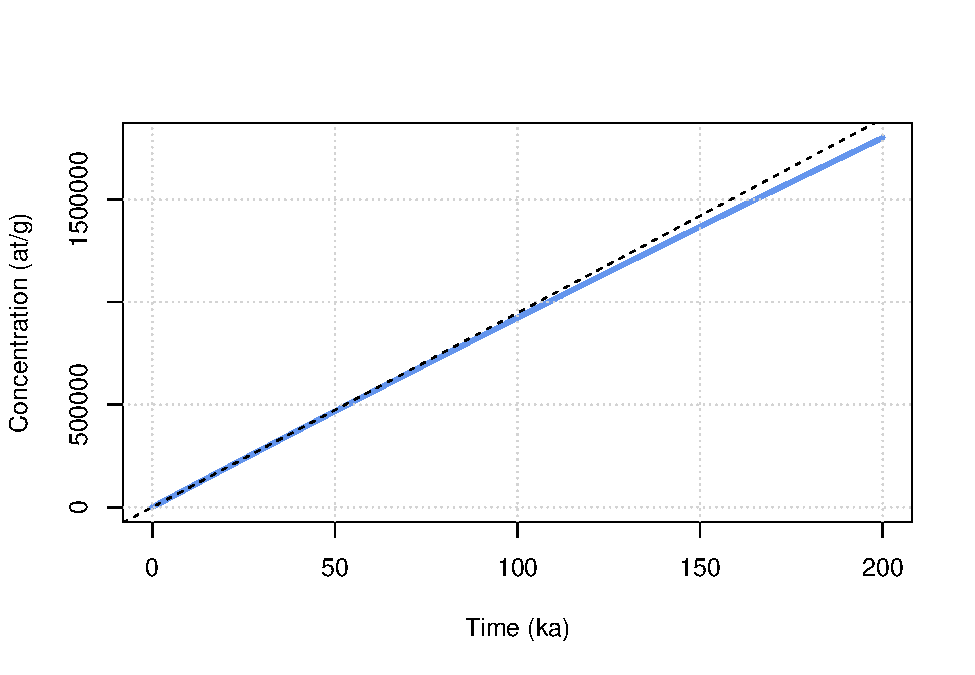
\includegraphics{_main_files/figure-latex/ck_5bis-1.pdf}

Start with zero erosion (\(\varepsilon=0\)), corresponding to the pure exposition of a surface.
We see here the progressive build-up of concentration though time and the establishment of balance between gains (production) and losses (denudation and decay) leading to the concentration plateau at steady state.

Two lines are added to the graph,

\begin{itemize}
\tightlist
\item
  The first one corresponds to the production slope \(\sum_i P_i\), how much nuclide you produce and how it would accumulate if you had no radioactive decay and no denudation.
\item
  The second one (horizontal) is the maximum value of concentration when steady state is achieved :
  \[ C_{max}=\sum_i \frac{P_i}{\frac{\rho \varepsilon}{\Lambda_i}+\lambda} \]
\end{itemize}

\begin{quote}
\textbf{TODO}
\end{quote}

\begin{itemize}
\tightlist
\item
  Change the maximum of the \texttt{t} vector until you see the influence of radioactive decay and the plateau.
\item
  Add some inheritance
\item
  Test the evolution with other nuclides (\(^{26}\)Al and \(^{14}\)C)
\end{itemize}

You can also play around with this build up using this Shiny App :

\url{http://shinyproxy.osupytheas.fr/simple_accumulation}

Now try to modify the \texttt{ero} (always keeping it is in g/cm\(^2\)/a) parameter above, to see its influence on time needed to reach steady state and the final concentration.

\hypertarget{two-end-member-situations}{%
\section{Two end-member situations}\label{two-end-member-situations}}

No we are going to build a summary plot showing the influence of both exposure and denudation.

\begin{Shaded}
\begin{Highlighting}[]
\NormalTok{altitude }\OtherTok{=} \DecValTok{1000} \CommentTok{\# elevation in m}
\NormalTok{latitude }\OtherTok{=} \DecValTok{45} \CommentTok{\# latitude in degrees}
\NormalTok{nuc }\OtherTok{=} \StringTok{"Be10"}
\NormalTok{P }\OtherTok{=} \FunctionTok{atm\_pressure}\NormalTok{(}\AttributeTok{alt=}\NormalTok{altitude,}\AttributeTok{model=}\StringTok{"stone2000"}\NormalTok{) }\CommentTok{\# compute atmospheric pressure at site}
\NormalTok{S }\OtherTok{=} \FunctionTok{scaling\_st}\NormalTok{(P,latitude) }\CommentTok{\# compute the scaling parameters according to Stone (2000)}
\NormalTok{t }\OtherTok{=}  \DecValTok{10}\SpecialCharTok{\^{}}\FunctionTok{seq}\NormalTok{(}\FunctionTok{log10}\NormalTok{(}\DecValTok{1}\NormalTok{),}\FunctionTok{log10}\NormalTok{(}\FloatTok{10e6}\NormalTok{),}\AttributeTok{length.out=}\DecValTok{1000}\NormalTok{) }\CommentTok{\# time vector, log{-}spaced!}
\CommentTok{\# calculation of the evolution of concentration for denudation = 0}
\NormalTok{C }\OtherTok{=} \FunctionTok{solv\_conc\_eul}\NormalTok{(}\DecValTok{0}\NormalTok{,}\DecValTok{0}\NormalTok{,t,}\DecValTok{0}\NormalTok{,prm[,nuc],S,Lambda) }\CommentTok{\# compute concentration for pure exposure}
\FunctionTok{plot}\NormalTok{(t,C,}\AttributeTok{type=}\StringTok{"l"}\NormalTok{,}\AttributeTok{col=}\StringTok{"cornflowerblue"}\NormalTok{,}\AttributeTok{lwd=}\DecValTok{3}\NormalTok{,}\AttributeTok{ylab=}\StringTok{"Concentration (at/g)"}\NormalTok{,}\AttributeTok{xlab=}\StringTok{"Time (a)"}\NormalTok{,}\AttributeTok{log=}\StringTok{"xy"}\NormalTok{)}
\FunctionTok{grid}\NormalTok{()}
\FunctionTok{text}\NormalTok{(}\FunctionTok{max}\NormalTok{(t),}\FunctionTok{max}\NormalTok{(C),}\DecValTok{0}\NormalTok{,}\AttributeTok{cex=}\FloatTok{0.5}\NormalTok{,}\AttributeTok{adj=}\DecValTok{0}\NormalTok{) }\CommentTok{\# label the curve}
\CommentTok{\# now we make the same computation for other denudation rates}
\NormalTok{ero }\OtherTok{=} \FunctionTok{c}\NormalTok{(}\DecValTok{1}\NormalTok{,}\DecValTok{10}\NormalTok{,}\DecValTok{100}\NormalTok{,}\DecValTok{1000}\NormalTok{) }\CommentTok{\# erosion vector in m/Ma}
\ControlFlowTok{for}\NormalTok{ (i }\ControlFlowTok{in} \DecValTok{1}\SpecialCharTok{:}\FunctionTok{length}\NormalTok{(ero))\{}
\NormalTok{  e }\OtherTok{=}\NormalTok{ ero[i] }\SpecialCharTok{*}\NormalTok{ (}\DecValTok{100}\SpecialCharTok{/}\FloatTok{1e6}\SpecialCharTok{*}\NormalTok{rho) }\CommentTok{\# convert denudation in g/cm2/a}
\NormalTok{  C }\OtherTok{=} \FunctionTok{solv\_conc\_eul}\NormalTok{(}\DecValTok{0}\NormalTok{,e,t,}\DecValTok{0}\NormalTok{,prm[,nuc],S,Lambda) }\CommentTok{\# compute concentration for pure exposure}
  \FunctionTok{lines}\NormalTok{(t,C,}\AttributeTok{col=}\StringTok{"cornflowerblue"}\NormalTok{,}\AttributeTok{lwd=}\DecValTok{3}\NormalTok{)}
  \FunctionTok{text}\NormalTok{(}\FunctionTok{max}\NormalTok{(t),}\FunctionTok{max}\NormalTok{(C),ero[i],}\AttributeTok{cex=}\FloatTok{0.5}\NormalTok{,}\AttributeTok{adj=}\DecValTok{0}\NormalTok{) }\CommentTok{\# label the curve}
\NormalTok{\}}
\end{Highlighting}
\end{Shaded}

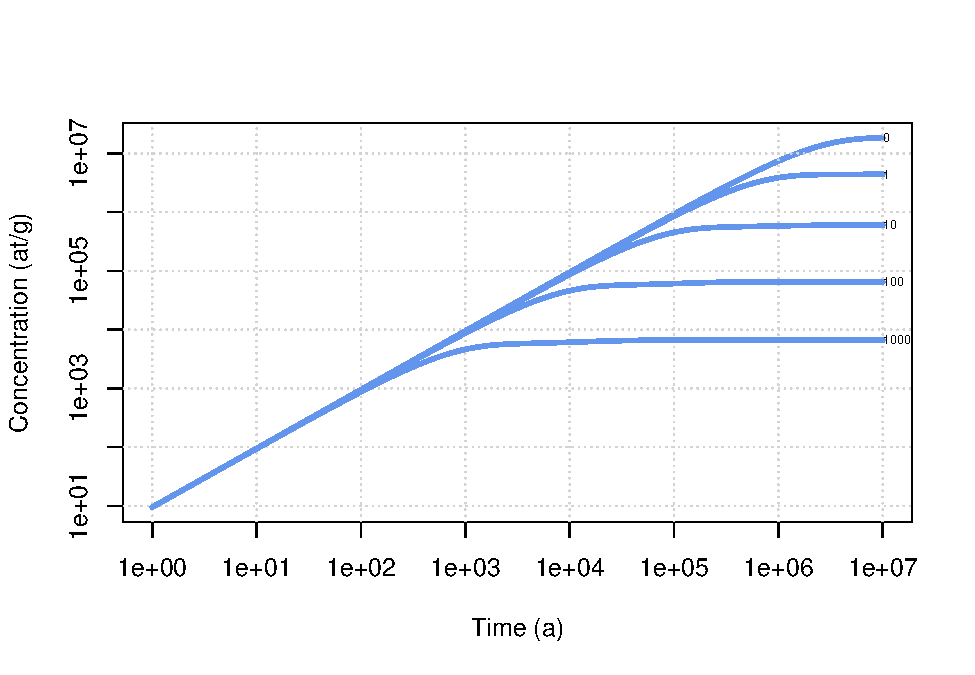
\includegraphics{_main_files/figure-latex/unnamed-chunk-16-1.pdf}

Note that this a log-log plot. It is probably one of the most important figure to keep in mind when analyzing TCN concentrations. It clearly shows the existence of two end-member situations when interpreting these concentrations, in terms of exposure age or denudation rates, and the transition between the two.

\begin{quote}
\textbf{TODO} Think about a bit about the following points
\end{quote}

\begin{itemize}
\tightlist
\item
  What are the key hypothesis made when interpreting a TCN concentration in terms of

  \begin{itemize}
  \tightlist
  \item
    exposure age
  \item
    surface denudation
  \end{itemize}
\item
  Can you think of geological/geomorphological situations where these hypotheses are violated?
\item
  Why are the plateau concentrations so different?
\item
  How is the time to reach the plateau changing and why?
\end{itemize}

\hypertarget{application-to-exposure-dating}{%
\chapter{Application to exposure dating}\label{application-to-exposure-dating}}

\hypertarget{back-to-the-evolution-of-concentration}{%
\section{Back to the evolution of concentration}\label{back-to-the-evolution-of-concentration}}

We first consider the evolution of concentration with time \(t\).
The computation will be carried out at the surface (\(z=0\)), but this could be done at any arbitrary depth.
We also consider that \(\varepsilon = 0\) and that there is no inheritance.
The starting equation above becomes, \[
C(t)=\sum_i \frac{P_i}{\lambda}(1-e^{-\lambda t})
\]
For the sake of the example we are going to compute that by hand, and compare with our results above obtained with the \texttt{solv\_conc\_eul} function,

\begin{Shaded}
\begin{Highlighting}[]
\CommentTok{\# set up}
\NormalTok{altitude }\OtherTok{=} \DecValTok{1000} \CommentTok{\# elevation in m}
\NormalTok{latitude }\OtherTok{=} \DecValTok{45} \CommentTok{\# latitude in degrees}
\NormalTok{nuc }\OtherTok{=} \StringTok{"Be10"}
\NormalTok{P }\OtherTok{=} \FunctionTok{atm\_pressure}\NormalTok{(}\AttributeTok{alt=}\NormalTok{altitude,}\AttributeTok{model=}\StringTok{"stone2000"}\NormalTok{) }\CommentTok{\# compute atmospheric pressure at site}
\NormalTok{S }\OtherTok{=} \FunctionTok{scaling\_st}\NormalTok{(P,latitude) }\CommentTok{\# compute the scaling parameters according to Stone (2000)}
\NormalTok{t }\OtherTok{=}  \FunctionTok{seq}\NormalTok{(}\DecValTok{0}\NormalTok{,}\FloatTok{200e3}\NormalTok{,}\AttributeTok{by=}\DecValTok{100}\NormalTok{) }\CommentTok{\# a vector containing time from 0 to 100 ka by 100 a steps}
\NormalTok{Pspal }\OtherTok{=}\NormalTok{ prm[}\DecValTok{1}\NormalTok{,nuc]}\SpecialCharTok{*}\NormalTok{S}\SpecialCharTok{$}\NormalTok{Nneutrons }\CommentTok{\# scaled spallation production rate in at/g/y (st scaling)}
\NormalTok{Pstop }\OtherTok{=}\NormalTok{ prm[}\DecValTok{2}\NormalTok{,nuc]}\SpecialCharTok{*}\NormalTok{S}\SpecialCharTok{$}\NormalTok{Nmuons }\CommentTok{\# scaled stopped muons  production rate in at/g/y}
\NormalTok{Pfast }\OtherTok{=}\NormalTok{ prm[}\DecValTok{3}\NormalTok{,nuc]}\SpecialCharTok{*}\NormalTok{S}\SpecialCharTok{$}\NormalTok{Nmuons }\CommentTok{\# scaled fast muons  production rate in at/g/y}
\NormalTok{lambda }\OtherTok{=}\NormalTok{ prm[}\DecValTok{4}\NormalTok{,nuc] }\CommentTok{\# radioactive decay (1/y)}
\NormalTok{C }\OtherTok{=}\NormalTok{ (Pspal }\SpecialCharTok{+}\NormalTok{ Pstop }\SpecialCharTok{+}\NormalTok{ Pfast) }\SpecialCharTok{/}\NormalTok{ lambda }\SpecialCharTok{*}\NormalTok{ (}\DecValTok{1}\SpecialCharTok{{-}}\FunctionTok{exp}\NormalTok{(}\SpecialCharTok{{-}}\NormalTok{lambda}\SpecialCharTok{*}\NormalTok{t))}
\FunctionTok{plot}\NormalTok{(t}\SpecialCharTok{/}\DecValTok{1000}\NormalTok{,C,}\AttributeTok{type=}\StringTok{"l"}\NormalTok{,}\AttributeTok{col=}\StringTok{"coral"}\NormalTok{,}\AttributeTok{lwd=}\DecValTok{3}\NormalTok{,}\AttributeTok{ylab=}\StringTok{"Concentration (at/g)"}\NormalTok{,}\AttributeTok{xlab=}\StringTok{"Time (ka)"}\NormalTok{)}
\FunctionTok{grid}\NormalTok{()}
\CommentTok{\# check if this is ok}
\NormalTok{C2 }\OtherTok{=} \FunctionTok{solv\_conc\_eul}\NormalTok{(}\DecValTok{0}\NormalTok{,}\DecValTok{0}\NormalTok{,t,}\DecValTok{0}\NormalTok{,prm[,nuc],S,Lambda) }\CommentTok{\# compute concentration for pure exposure}
\FunctionTok{lines}\NormalTok{(t}\SpecialCharTok{/}\DecValTok{1000}\NormalTok{,C2,}\AttributeTok{lty=}\DecValTok{2}\NormalTok{)}
\end{Highlighting}
\end{Shaded}

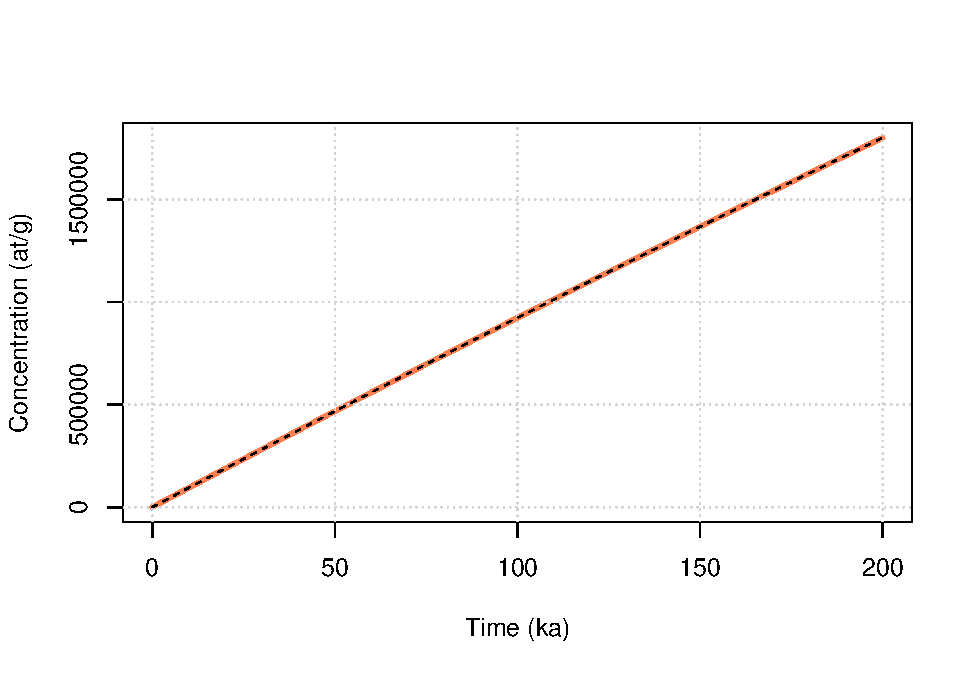
\includegraphics{_main_files/figure-latex/`-1.pdf}

On thing to note in this graph is that time \(t\) is expressed as \emph{time elapsed since start of exposure}, which we can not directly translate into the age BP, when dealing with radioactive decay and time variations in production rate.

\hypertarget{interpretation-in-terms-of-exposure-ages}{%
\section{Interpretation in terms of exposure ages}\label{interpretation-in-terms-of-exposure-ages}}

We are no going to make some simple calculations to convert our concentrations in terms of exposure age.
It basically solving for \(t\) the equation \(C_{mod}(t) = C_{mes}\). The left hand side is our modelled concentration, obtained for example with ou simple Eulerian model (\texttt{solv\_conc\_eul}), where we need to keep in mind all the hypotheses we make (\(z=0\), \(\varepsilon=0\), \(C_0=0\))

We are going to use an example from Protin et al. (\protect\hyperlink{ref-protin2019climatic}{2019}), using sample \emph{ARG-16-9}. Here are the characteristics of this sample.

\begin{Shaded}
\begin{Highlighting}[]
\NormalTok{rho }\OtherTok{=} \FloatTok{2.7}
\NormalTok{altitude }\OtherTok{=} \DecValTok{2252} \CommentTok{\# elevation in m}
\NormalTok{latitude }\OtherTok{=} \FloatTok{45.97} \CommentTok{\# latitude in degrees}
\NormalTok{longitude }\OtherTok{=} \FloatTok{6.96} \CommentTok{\# longitude in degrees}
\NormalTok{Ss }\OtherTok{=} \FloatTok{0.939}\SpecialCharTok{*}\FunctionTok{exp}\NormalTok{(}\SpecialCharTok{{-}}\FloatTok{2.6}\SpecialCharTok{*}\NormalTok{rho}\SpecialCharTok{/}\NormalTok{Lambda[}\DecValTok{1}\NormalTok{]) }\CommentTok{\# factor accounting for topographic shielding and sample thickness}
\NormalTok{Cmes }\OtherTok{=} \FloatTok{26.8e4} \CommentTok{\# measured concentration (at/g)}
\NormalTok{Cmes\_e }\OtherTok{=} \FloatTok{1.3e4}
\CommentTok{\#}
\NormalTok{P }\OtherTok{=} \FunctionTok{atm\_pressure}\NormalTok{(}\AttributeTok{alt=}\NormalTok{altitude,}\AttributeTok{lat=}\NormalTok{latitude,}\AttributeTok{lon=}\NormalTok{longitude,}\AttributeTok{model=}\StringTok{"era40"}\NormalTok{) }\CommentTok{\# compute atmospheric pressure at site}
\NormalTok{S }\OtherTok{=} \FunctionTok{scaling\_st}\NormalTok{(P,latitude) }\CommentTok{\# compute the scaling parameters according to Stone (2000)}
\end{Highlighting}
\end{Shaded}

Now, for example we can make some guess about the exposure age and see what is the difference with the measured concentration.

\begin{Shaded}
\begin{Highlighting}[]
\NormalTok{age }\OtherTok{=} \FloatTok{10e3} \CommentTok{\# a }
\NormalTok{Cmod }\OtherTok{=} \FunctionTok{solv\_conc\_eul}\NormalTok{(}\DecValTok{0}\NormalTok{,}\DecValTok{0}\NormalTok{,age,}\DecValTok{0}\NormalTok{,prm[,}\StringTok{"Be10"}\NormalTok{],S}\SpecialCharTok{*}\NormalTok{Ss,Lambda) }\CommentTok{\# compute concentration}
\end{Highlighting}
\end{Shaded}

We could try make \texttt{Cmod} equal to \texttt{Cmes} by trial and error, but we can be more systematic,

\begin{Shaded}
\begin{Highlighting}[]
\NormalTok{age }\OtherTok{=} \FunctionTok{seq}\NormalTok{(}\DecValTok{0}\NormalTok{,}\FloatTok{20e3}\NormalTok{,}\AttributeTok{by=}\DecValTok{10}\NormalTok{)}
\NormalTok{Cmod }\OtherTok{=} \FunctionTok{rep}\NormalTok{(}\ConstantTok{NA}\NormalTok{,}\FunctionTok{length}\NormalTok{(age))}
\ControlFlowTok{for}\NormalTok{ (i }\ControlFlowTok{in} \DecValTok{1}\SpecialCharTok{:}\FunctionTok{length}\NormalTok{(age))\{}
\NormalTok{  Cmod[i] }\OtherTok{=} \FunctionTok{solv\_conc\_eul}\NormalTok{(}\DecValTok{0}\NormalTok{,}\DecValTok{0}\NormalTok{,age[i],}\DecValTok{0}\NormalTok{,prm[,}\StringTok{"Be10"}\NormalTok{],S}\SpecialCharTok{*}\NormalTok{Ss,Lambda) }\CommentTok{\# compute concentration}
\NormalTok{\}}
\NormalTok{imin }\OtherTok{=} \FunctionTok{which.min}\NormalTok{(}\FunctionTok{abs}\NormalTok{(Cmod}\SpecialCharTok{{-}}\NormalTok{Cmes))}
\NormalTok{res }\OtherTok{=}\NormalTok{ age[imin]}
\FunctionTok{plot}\NormalTok{(age,Cmod}\SpecialCharTok{{-}}\NormalTok{Cmes,}\AttributeTok{type=}\StringTok{"l"}\NormalTok{,}\AttributeTok{main=}\FunctionTok{paste}\NormalTok{(res,}\StringTok{"a BP"}\NormalTok{),}\AttributeTok{col=}\StringTok{"coral"}\NormalTok{,}\AttributeTok{lwd=}\DecValTok{2}\NormalTok{)}
\FunctionTok{abline}\NormalTok{(}\AttributeTok{h=}\DecValTok{0}\NormalTok{)}
\FunctionTok{abline}\NormalTok{(}\AttributeTok{v=}\NormalTok{res)}
\end{Highlighting}
\end{Shaded}

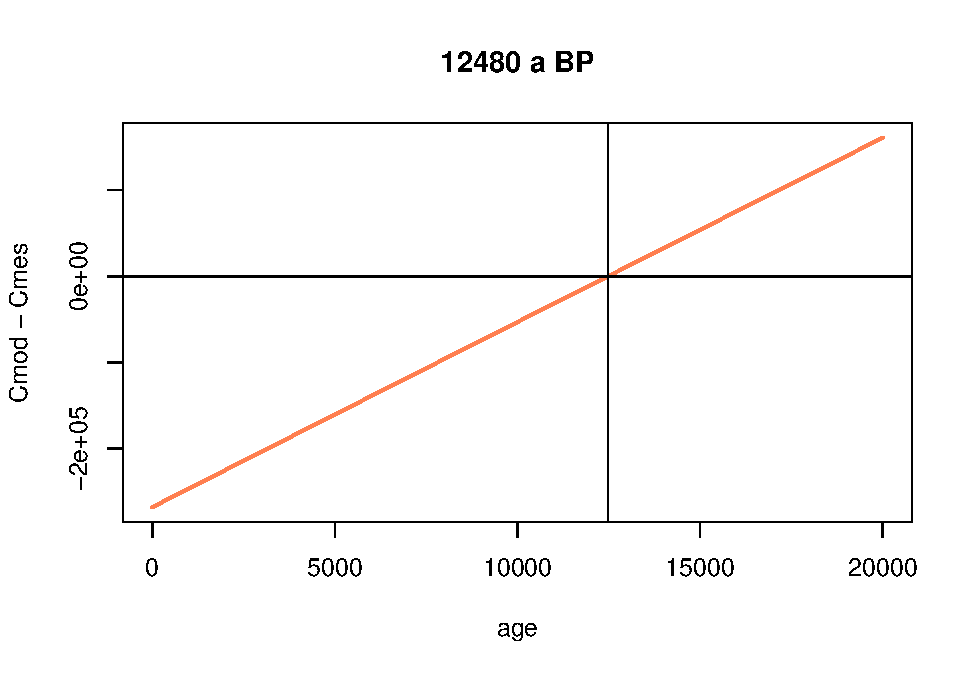
\includegraphics{_main_files/figure-latex/unnamed-chunk-20-1.pdf}

\begin{quote}
\textbf{TODO} Compare with the age from table 1 from Protin et al. (\protect\hyperlink{ref-protin2019climatic}{2019}). Comment about the possible causes for the differences?
\end{quote}

We can be even more efficient by using an simple optimization approach to solve \(C_{mod}(t) = C_{mes}\), using the built in \texttt{optimize} function. We just define a function to be optimized (search of minimum) and launch a search over an age range. We are looking for the minimum value of \(|C_{mod}-C_{mes}|\)

\begin{Shaded}
\begin{Highlighting}[]
\NormalTok{fun\_opt }\OtherTok{\textless{}{-}}\ControlFlowTok{function}\NormalTok{(t,Cmes,prm,S,Lambda)\{}
\NormalTok{  Cmod }\OtherTok{=} \FunctionTok{solv\_conc\_eul}\NormalTok{(}\DecValTok{0}\NormalTok{,}\DecValTok{0}\NormalTok{,t,}\DecValTok{0}\NormalTok{,prm[,}\StringTok{"Be10"}\NormalTok{],S,Lambda)}
  \FunctionTok{return}\NormalTok{(}\FunctionTok{abs}\NormalTok{(Cmod}\SpecialCharTok{{-}}\NormalTok{Cmes))}
\NormalTok{\}}
\NormalTok{res }\OtherTok{=} \FunctionTok{optimize}\NormalTok{(fun\_opt,}\FunctionTok{c}\NormalTok{(}\DecValTok{0}\NormalTok{,}\FloatTok{50e3}\NormalTok{),Cmes,prm,S}\SpecialCharTok{*}\NormalTok{Ss,Lambda)}
\FunctionTok{print}\NormalTok{(res)}
\end{Highlighting}
\end{Shaded}

\begin{verbatim}
## $minimum
## [1] 12478.57
## 
## $objective
## [1] 0.0008513347
\end{verbatim}

\hypertarget{time-varying-production-rates}{%
\section{Time varying production rates}\label{time-varying-production-rates}}

We are now going back to the time varying-scaling parameters

\begin{Shaded}
\begin{Highlighting}[]
\NormalTok{data }\OtherTok{=} \FunctionTok{data.frame}\NormalTok{(}\AttributeTok{t1=}\FunctionTok{seq}\NormalTok{(}\DecValTok{0}\NormalTok{,}\FloatTok{50e3}\NormalTok{,}\AttributeTok{length.out=}\DecValTok{2000}\NormalTok{)) }\CommentTok{\# we build a dataframe to store results}
\NormalTok{data}\SpecialCharTok{$}\NormalTok{t2 }\OtherTok{=} \FunctionTok{max}\NormalTok{(data}\SpecialCharTok{$}\NormalTok{t1) }\SpecialCharTok{{-}}\NormalTok{ data}\SpecialCharTok{$}\NormalTok{t1 }\CommentTok{\# time BP}
\NormalTok{data}\SpecialCharTok{$}\NormalTok{vdm }\OtherTok{=} \FunctionTok{get\_vdm}\NormalTok{(data}\SpecialCharTok{$}\NormalTok{t2,}\AttributeTok{model=}\StringTok{"musch"}\NormalTok{)}
\NormalTok{data}\SpecialCharTok{$}\NormalTok{rc }\OtherTok{=} \FunctionTok{vdm2rc}\NormalTok{(data}\SpecialCharTok{$}\NormalTok{vdm,latitude,}\AttributeTok{model=}\StringTok{"elsasser54"}\NormalTok{)}
\NormalTok{data}\SpecialCharTok{$}\NormalTok{lm }\OtherTok{=} \FunctionTok{scaling\_lm}\NormalTok{(P,data}\SpecialCharTok{$}\NormalTok{rc)}
\FunctionTok{plot}\NormalTok{(data}\SpecialCharTok{$}\NormalTok{t2,data}\SpecialCharTok{$}\NormalTok{lm,}\AttributeTok{type=}\StringTok{"l"}\NormalTok{,}\AttributeTok{xlab=}\StringTok{"Age BP (a)"}\NormalTok{,}\AttributeTok{ylab=}\StringTok{"Scaling factor"}\NormalTok{)}
\FunctionTok{abline}\NormalTok{(}\AttributeTok{h=}\NormalTok{S}\SpecialCharTok{$}\NormalTok{Nneutrons,}\AttributeTok{col=}\StringTok{"red"}\NormalTok{)}
\FunctionTok{abline}\NormalTok{(}\AttributeTok{h=}\FunctionTok{mean}\NormalTok{(data}\SpecialCharTok{$}\NormalTok{lm),}\AttributeTok{lty=}\DecValTok{2}\NormalTok{)}
\end{Highlighting}
\end{Shaded}

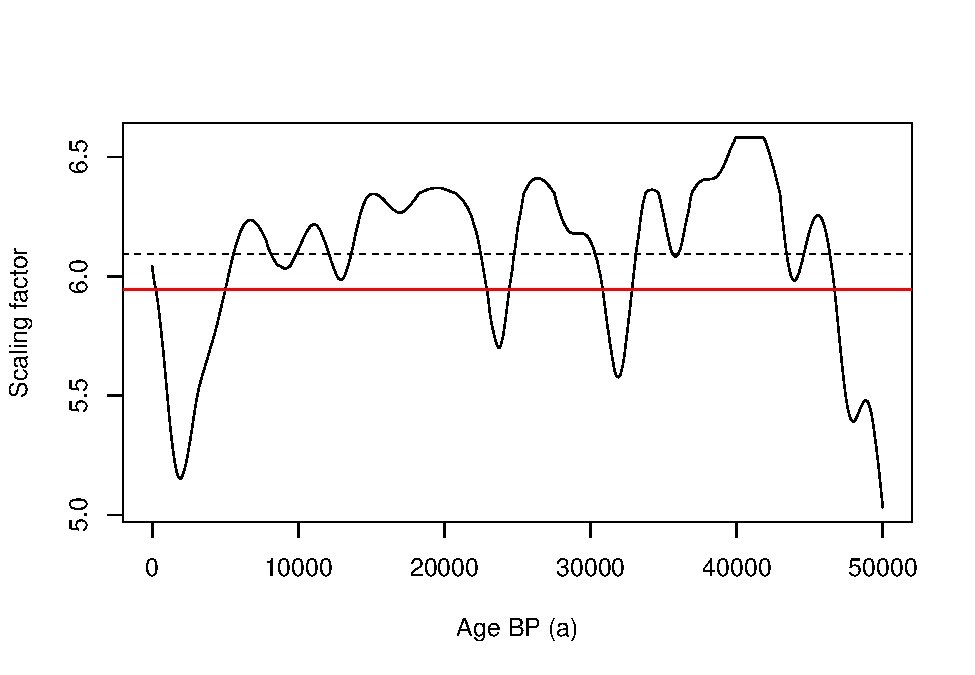
\includegraphics{_main_files/figure-latex/unnamed-chunk-22-1.pdf}

In this case we can not use the same equations for the evolution of TCN concentration as above, because we need to account for \(P(t)\). We are going to use,
\[C_{mod}(t) = \int_0^t P(t)e^{-\lambda t}dt\]
Note : it is usually considered that production by muons is much less affected than that by neutrons by the magnetic field variations.

Below we first compare how the concentration evolves through time with the two approaches.

\begin{Shaded}
\begin{Highlighting}[]
\FunctionTok{library}\NormalTok{(pracma) }\CommentTok{\# useful library containing the cumtrapz function for trapezoidal integration}
\NormalTok{data}\SpecialCharTok{$}\NormalTok{C1 }\OtherTok{=} \FunctionTok{solv\_conc\_eul}\NormalTok{(}\DecValTok{0}\NormalTok{,}\DecValTok{0}\NormalTok{,data}\SpecialCharTok{$}\NormalTok{t1,}\DecValTok{0}\NormalTok{,prm,S}\SpecialCharTok{*}\NormalTok{Ss,Lambda) }
\NormalTok{data}\SpecialCharTok{$}\NormalTok{C2 }\OtherTok{=} \FunctionTok{cumtrapz}\NormalTok{(data}\SpecialCharTok{$}\NormalTok{t1,(prm[}\DecValTok{1}\NormalTok{]}\SpecialCharTok{*}\NormalTok{data}\SpecialCharTok{$}\NormalTok{lm}\SpecialCharTok{*}\NormalTok{Ss}\SpecialCharTok{+}\NormalTok{(prm[}\DecValTok{2}\NormalTok{,}\StringTok{"Be10"}\NormalTok{] }\SpecialCharTok{+}\NormalTok{ prm[}\DecValTok{3}\NormalTok{,}\StringTok{"Be10"}\NormalTok{])}\SpecialCharTok{*}\NormalTok{Ss}\SpecialCharTok{*}\NormalTok{S}\SpecialCharTok{$}\NormalTok{Nmuons)}\SpecialCharTok{*}\NormalTok{(}\FunctionTok{exp}\NormalTok{(}\SpecialCharTok{{-}}\NormalTok{prm[}\StringTok{"lambda"}\NormalTok{,}\StringTok{\textquotesingle{}Be10\textquotesingle{}}\NormalTok{]}\SpecialCharTok{*}\NormalTok{data}\SpecialCharTok{$}\NormalTok{t1)))[,}\DecValTok{1}\NormalTok{] }
\FunctionTok{plot}\NormalTok{(data}\SpecialCharTok{$}\NormalTok{t1,data}\SpecialCharTok{$}\NormalTok{C1,}\AttributeTok{type=}\StringTok{"l"}\NormalTok{,}\AttributeTok{xlab=}\StringTok{"time (a)"}\NormalTok{,}\AttributeTok{ylab=}\StringTok{"Concentration (at/g)"}\NormalTok{,}\AttributeTok{col=}\StringTok{"cyan4"}\NormalTok{)}
\FunctionTok{lines}\NormalTok{(data}\SpecialCharTok{$}\NormalTok{t1,data}\SpecialCharTok{$}\NormalTok{C2,}\AttributeTok{col=}\StringTok{"darkgoldenrod2"}\NormalTok{)}
\FunctionTok{legend}\NormalTok{(}\StringTok{"topleft"}\NormalTok{,}\FunctionTok{c}\NormalTok{(}\StringTok{"st"}\NormalTok{,}\StringTok{"lm"}\NormalTok{),}\AttributeTok{lty=}\DecValTok{1}\NormalTok{,}\AttributeTok{col=}\FunctionTok{c}\NormalTok{(}\StringTok{"cyan4"}\NormalTok{, }\StringTok{"darkgoldenrod2"}\NormalTok{))}
\end{Highlighting}
\end{Shaded}

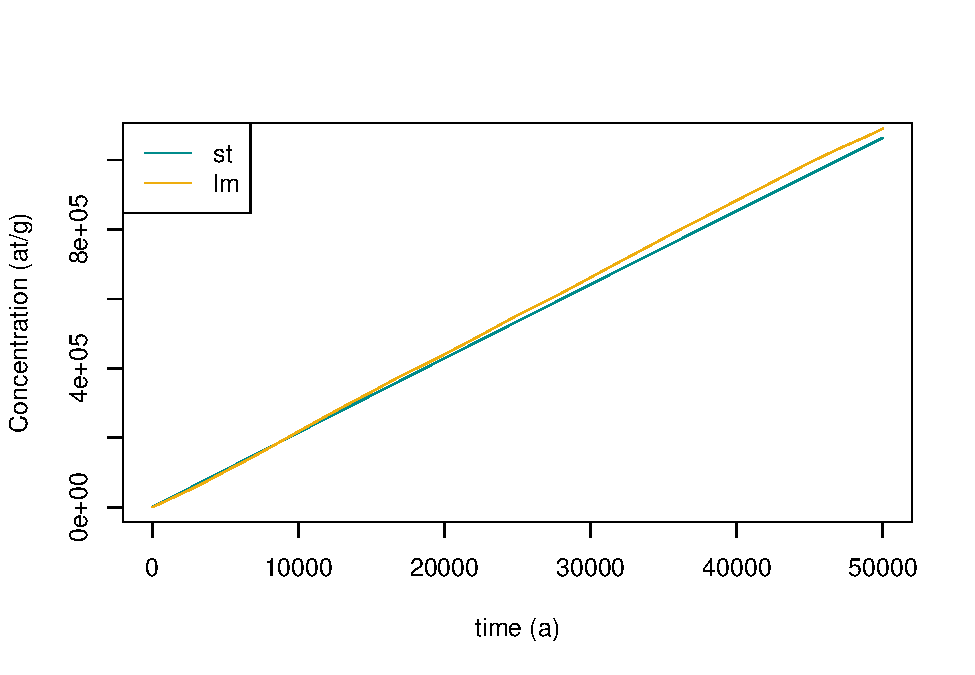
\includegraphics{_main_files/figure-latex/unnamed-chunk-23-1.pdf}

We can solve solve \(|C_{mod}-C_{mes}|\) for \(t\) with the same approach as the \texttt{st} case,

\begin{Shaded}
\begin{Highlighting}[]
\NormalTok{compute\_C}\OtherTok{\textless{}{-}}\ControlFlowTok{function}\NormalTok{(t1,prm,P,lat,Lambda,S)\{}
\NormalTok{  data }\OtherTok{=} \FunctionTok{data.frame}\NormalTok{(}\AttributeTok{t1=}\FunctionTok{seq}\NormalTok{(}\DecValTok{0}\NormalTok{,t1,}\AttributeTok{length.out=}\DecValTok{1000}\NormalTok{)) }\CommentTok{\# we build a dataframe to store results}
\NormalTok{  data}\SpecialCharTok{$}\NormalTok{t2 }\OtherTok{=} \FunctionTok{max}\NormalTok{(data}\SpecialCharTok{$}\NormalTok{t1) }\SpecialCharTok{{-}}\NormalTok{ data}\SpecialCharTok{$}\NormalTok{t1 }\CommentTok{\# time BP}
\NormalTok{  data}\SpecialCharTok{$}\NormalTok{vdm }\OtherTok{=} \FunctionTok{get\_vdm}\NormalTok{(data}\SpecialCharTok{$}\NormalTok{t2,}\AttributeTok{model=}\StringTok{"musch"}\NormalTok{)}
\NormalTok{  data}\SpecialCharTok{$}\NormalTok{rc }\OtherTok{=} \FunctionTok{vdm2rc}\NormalTok{(data}\SpecialCharTok{$}\NormalTok{vdm,lat,}\AttributeTok{model=}\StringTok{"elsasser54"}\NormalTok{)}
\NormalTok{  data}\SpecialCharTok{$}\NormalTok{lm }\OtherTok{=} \FunctionTok{scaling\_lm}\NormalTok{(P,data}\SpecialCharTok{$}\NormalTok{rc)}
\NormalTok{  Cmod }\OtherTok{=} \FunctionTok{trapz}\NormalTok{(data}\SpecialCharTok{$}\NormalTok{t1,(prm[}\DecValTok{1}\NormalTok{,}\StringTok{"Be10"}\NormalTok{]}\SpecialCharTok{*}\NormalTok{data}\SpecialCharTok{$}\NormalTok{lm}\SpecialCharTok{+}\NormalTok{(prm[}\DecValTok{2}\NormalTok{,}\StringTok{"Be10"}\NormalTok{] }\SpecialCharTok{+}\NormalTok{ prm[}\DecValTok{3}\NormalTok{,}\StringTok{"Be10"}\NormalTok{])}\SpecialCharTok{*}\NormalTok{S}\SpecialCharTok{$}\NormalTok{Nmuons)}\SpecialCharTok{*}\NormalTok{(}\FunctionTok{exp}\NormalTok{(}\SpecialCharTok{{-}}\NormalTok{prm[}\StringTok{"lambda"}\NormalTok{,}\StringTok{\textquotesingle{}Be10\textquotesingle{}}\NormalTok{]}\SpecialCharTok{*}\NormalTok{data}\SpecialCharTok{$}\NormalTok{t2)))}
  \FunctionTok{return}\NormalTok{(Cmod)}
\NormalTok{\}}

\NormalTok{fun\_opt2 }\OtherTok{\textless{}{-}}\ControlFlowTok{function}\NormalTok{(t1,Cmes,prm,P,lat,Lambda,S)\{}
\NormalTok{  Cmod }\OtherTok{=}  \FunctionTok{compute\_C}\NormalTok{(t1,prm,P,lat,Lambda,S)}
  \FunctionTok{return}\NormalTok{(}\FunctionTok{abs}\NormalTok{(Cmod}\SpecialCharTok{{-}}\NormalTok{Cmes))}
\NormalTok{\}}

\NormalTok{  P }\OtherTok{=} \FunctionTok{atm\_pressure}\NormalTok{(}\AttributeTok{alt=}\NormalTok{altitude,}\AttributeTok{lat=}\NormalTok{latitude,}\AttributeTok{lon=}\NormalTok{longitude,}\AttributeTok{model=}\StringTok{"era40"}\NormalTok{) }\CommentTok{\# compute atmospheric pressure at site}
\NormalTok{  S }\OtherTok{=} \FunctionTok{scaling\_st}\NormalTok{(P,latitude) }\CommentTok{\# compute the scaling parameters according to Stone (2000)}
\NormalTok{  res }\OtherTok{=} \FunctionTok{optimize}\NormalTok{(fun\_opt2,}\FunctionTok{c}\NormalTok{(}\DecValTok{0}\NormalTok{,}\FloatTok{50e3}\NormalTok{),Cmes,prm,P,latitude,Lambda,S}\SpecialCharTok{*}\NormalTok{Ss)}
\FunctionTok{print}\NormalTok{(res)}
\end{Highlighting}
\end{Shaded}

\begin{verbatim}
## $minimum
## [1] 11343.93
## 
## $objective
## [1] 0.0003504902
\end{verbatim}

Caveat we did those calculation using a number of simplification and numerical shortcuts \ldots.

\hypertarget{dealing-with-uncertainties}{%
\section{Dealing with uncertainties}\label{dealing-with-uncertainties}}

\hypertarget{application-to-denudation-rate-measurements}{%
\chapter{Application to denudation rate measurements}\label{application-to-denudation-rate-measurements}}

\hypertarget{concentration---denudation-rate-relationship}{%
\section{Concentration - denudation rate relationship}\label{concentration---denudation-rate-relationship}}

Now we are going to consider the evolution of concentration with denudation rate \(\varepsilon\).
The computation will be carried out at the surface (\(z=0\)), but this could be done at any arbitrary depth.
We will consider that \(t=+\infty\) and that we have reached the plateau concentration.
The key equation is now,
\[C=\sum_i \frac{P_i}{\frac{\rho \varepsilon}{\Lambda_i}+\lambda}\]

Which simplifies to \(C\approx\frac{P_i \Lambda_i}{\rho \varepsilon}\) if we neglect radioactive decay.

Let's define the usual parameters.

\begin{Shaded}
\begin{Highlighting}[]
\NormalTok{altitude }\OtherTok{=} \DecValTok{1000} \CommentTok{\# elevation in m}
\NormalTok{latitude }\OtherTok{=} \DecValTok{45} \CommentTok{\# latitude in degrees}
\NormalTok{rho }\OtherTok{=} \FloatTok{2.7}
\FunctionTok{data}\NormalTok{(prm)}
\FunctionTok{data}\NormalTok{(Lambda)}
\NormalTok{P }\OtherTok{=} \FunctionTok{atm\_pressure}\NormalTok{(}\AttributeTok{alt=}\NormalTok{altitude,}\AttributeTok{model=}\StringTok{"stone2000"}\NormalTok{) }\CommentTok{\# compute atmospheric pressure at site}
\NormalTok{S }\OtherTok{=} \FunctionTok{scaling\_st}\NormalTok{(P,latitude) }\CommentTok{\# compute the scaling parameters according to Stone (2000)}
\end{Highlighting}
\end{Shaded}

Now compute the steady-state concentration for a range of denudation rates.

\begin{Shaded}
\begin{Highlighting}[]
\NormalTok{nuc }\OtherTok{=} \StringTok{"Be10"}
\NormalTok{ero }\OtherTok{=} \DecValTok{10}\SpecialCharTok{\^{}}\FunctionTok{seq}\NormalTok{(}\FunctionTok{log10}\NormalTok{(}\FloatTok{0.1}\NormalTok{),}\FunctionTok{log10}\NormalTok{(}\DecValTok{1000}\NormalTok{),}\AttributeTok{length.out =} \DecValTok{100}\NormalTok{) }\SpecialCharTok{*} \DecValTok{100}\SpecialCharTok{/}\FloatTok{1e6}\SpecialCharTok{*}\NormalTok{rho }\CommentTok{\# a log{-}spaced vector for denudation rate expressed in m/Ma and converted in g/cm2/a}
\NormalTok{age }\OtherTok{=}  \ConstantTok{Inf} \CommentTok{\# infinite age}
\NormalTok{z }\OtherTok{=} \DecValTok{0} \SpecialCharTok{*}\NormalTok{ rho }\CommentTok{\# depth at which we are going to perform the calculation (cm converted to g/cm2)}
\NormalTok{C0 }\OtherTok{=} \DecValTok{0} \CommentTok{\# inherited concentration}
\NormalTok{C }\OtherTok{=} \FunctionTok{solv\_conc\_eul}\NormalTok{(z,ero,age,C0,prm[,nuc],S,Lambda) }\CommentTok{\# compute concentration}
\FunctionTok{plot}\NormalTok{(ero}\SpecialCharTok{/}\DecValTok{100}\SpecialCharTok{*}\FloatTok{1e6}\SpecialCharTok{/}\NormalTok{rho,C,}\AttributeTok{col=}\StringTok{"lawngreen"}\NormalTok{,}\AttributeTok{log=}\StringTok{"xy"}\NormalTok{,}\AttributeTok{type=}\StringTok{"l"}\NormalTok{,}\AttributeTok{lwd=}\DecValTok{3}\NormalTok{,}\AttributeTok{ylab=}\StringTok{"Concentration (at/g)"}\NormalTok{,}\AttributeTok{xlab=}\StringTok{"Denudation rate (m/Ma)"}\NormalTok{)}
\FunctionTok{grid}\NormalTok{()}
\CommentTok{\# what happens if we neglect radioactive decay}
\NormalTok{Prod }\OtherTok{=} \FunctionTok{c}\NormalTok{(prm[}\DecValTok{1}\NormalTok{,nuc]}\SpecialCharTok{*}\NormalTok{S}\SpecialCharTok{$}\NormalTok{Nneutrons,prm[}\DecValTok{2}\NormalTok{,nuc]}\SpecialCharTok{*}\NormalTok{S}\SpecialCharTok{$}\NormalTok{Nmuons,prm[}\DecValTok{3}\NormalTok{,nuc]}\SpecialCharTok{*}\NormalTok{S}\SpecialCharTok{$}\NormalTok{Nmuons) }\CommentTok{\# scaled production vector (defined for the sake of clarity of the expressions below)}
\NormalTok{lambda }\OtherTok{=}\NormalTok{ prm[}\DecValTok{4}\NormalTok{,nuc] }\CommentTok{\# radioactive decay}
\NormalTok{C2 }\OtherTok{=}\NormalTok{ prm[}\DecValTok{1}\NormalTok{,nuc]}\SpecialCharTok{*}\NormalTok{S}\SpecialCharTok{$}\NormalTok{Nneutrons}\SpecialCharTok{*}\NormalTok{Lambda[}\DecValTok{1}\NormalTok{]}\SpecialCharTok{/}\NormalTok{ero }\SpecialCharTok{+}\NormalTok{ prm[}\DecValTok{2}\NormalTok{,nuc]}\SpecialCharTok{*}\NormalTok{S}\SpecialCharTok{$}\NormalTok{Nmuons}\SpecialCharTok{*}\NormalTok{Lambda[}\DecValTok{2}\NormalTok{]}\SpecialCharTok{/}\NormalTok{ero }\SpecialCharTok{+}\NormalTok{ prm[}\DecValTok{3}\NormalTok{,nuc]}\SpecialCharTok{*}\NormalTok{S}\SpecialCharTok{$}\NormalTok{Nmuons}\SpecialCharTok{*}\NormalTok{Lambda[}\DecValTok{3}\NormalTok{]}\SpecialCharTok{/}\NormalTok{ero    }
\FunctionTok{lines}\NormalTok{(ero}\SpecialCharTok{/}\DecValTok{100}\SpecialCharTok{*}\FloatTok{1e6}\SpecialCharTok{/}\NormalTok{rho,C2,}\AttributeTok{lty=}\DecValTok{2}\NormalTok{)}
\end{Highlighting}
\end{Shaded}

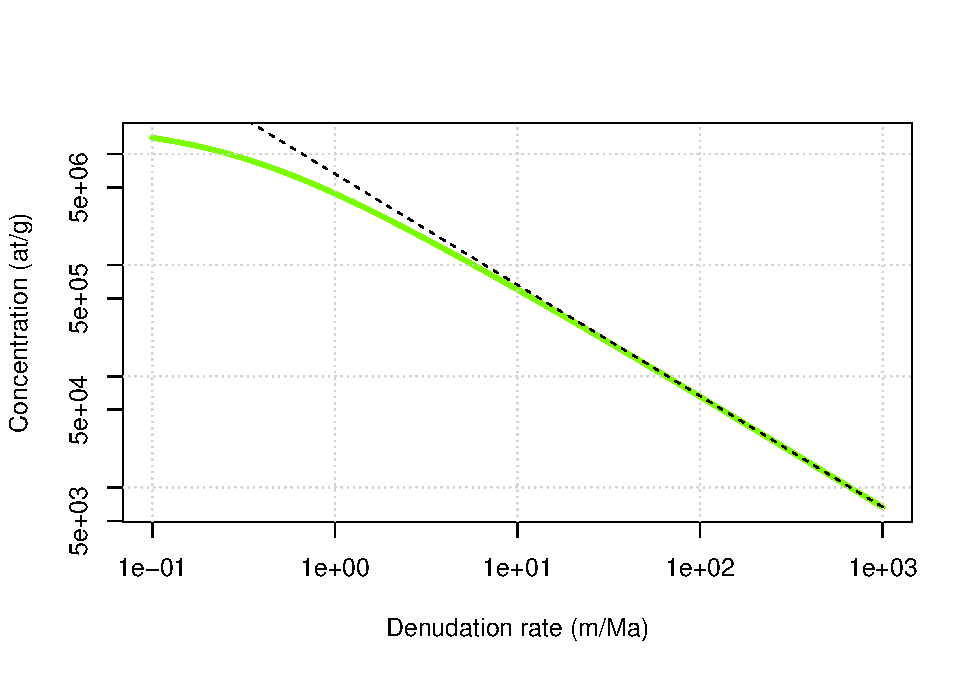
\includegraphics{_main_files/figure-latex/unnamed-chunk-27-1.pdf}

This figure (log-scales on both axes) highlights the strong inverse relationship, at steady-state, between denudation rate (\(\varepsilon\)) and concentration (\(C\)), which is the foundation of many geomorphological studies trying to establish landscape evolution rates.
Note the change in the relationship at very low denudation rates, which corresponds to the situation where the effects of radioactive decay become predominant.

\begin{quote}
\textbf{TODO} Over what range of denudation rates it is reasonable to neglect radioactive decay? What kind of geological context could it correspond to?
\end{quote}

A simple way to answer this question would be to compute the relative difference between the computed concentrations

\begin{Shaded}
\begin{Highlighting}[]
\NormalTok{error }\OtherTok{=} \FunctionTok{abs}\NormalTok{(C}\SpecialCharTok{{-}}\NormalTok{C2)}\SpecialCharTok{/}\NormalTok{C}\SpecialCharTok{*}\DecValTok{100}
\FunctionTok{plot}\NormalTok{(ero}\SpecialCharTok{/}\DecValTok{100}\SpecialCharTok{*}\FloatTok{1e6}\SpecialCharTok{/}\NormalTok{rho,error,}\AttributeTok{log=}\StringTok{"xy"}\NormalTok{,}\AttributeTok{type=}\StringTok{"l"}\NormalTok{,}\AttributeTok{ylab=}\StringTok{"Relative error (\%)"}\NormalTok{,}\AttributeTok{xlab=}\StringTok{"Denudation rate (m/Ma)"}\NormalTok{)}
\end{Highlighting}
\end{Shaded}

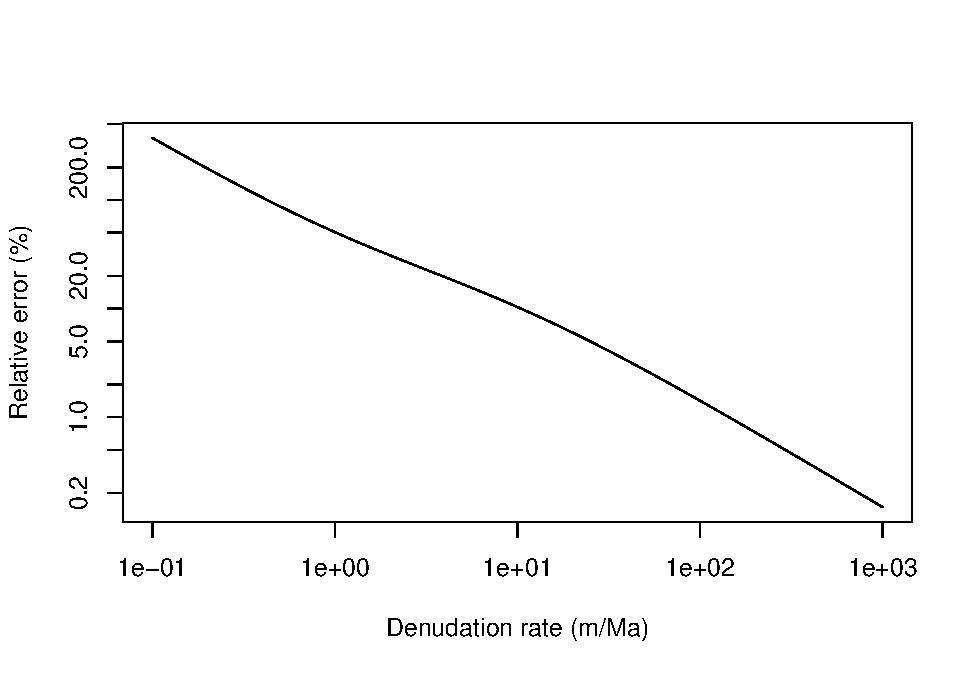
\includegraphics{_main_files/figure-latex/unnamed-chunk-28-1.pdf}

\hypertarget{integration-time-scale}{%
\section{Integration time scale}\label{integration-time-scale}}

\hypertarget{on-the-importance-of-muons}{%
\section{On the importance of muons}\label{on-the-importance-of-muons}}

For \(^{10}\)Be the muonic represent a very small fraction of surface production :

\begin{Shaded}
\begin{Highlighting}[]
\NormalTok{nuc }\OtherTok{=} \StringTok{"Be10"}
\NormalTok{f }\OtherTok{=}\NormalTok{ (prm[}\DecValTok{2}\NormalTok{,nuc]}\SpecialCharTok{+}\NormalTok{prm[}\DecValTok{3}\NormalTok{,nuc])}\SpecialCharTok{/}\FunctionTok{sum}\NormalTok{(prm[}\DecValTok{1}\SpecialCharTok{:}\DecValTok{3}\NormalTok{,nuc])}\SpecialCharTok{*}\DecValTok{100}
\FunctionTok{paste}\NormalTok{(}\StringTok{"For"}\NormalTok{,nuc,}\StringTok{"muons represent"}\NormalTok{,}\FunctionTok{round}\NormalTok{(f,}\DecValTok{1}\NormalTok{),}\StringTok{"\% of SLHL surface production"}\NormalTok{)}
\end{Highlighting}
\end{Shaded}

\begin{verbatim}
## [1] "For Be10 muons represent 1.3 % of SLHL surface production"
\end{verbatim}

\begin{Shaded}
\begin{Highlighting}[]
\NormalTok{col\_sp }\OtherTok{=} \StringTok{"deepskyblue"}
\NormalTok{col\_sm }\OtherTok{=} \StringTok{"indianred1"}
\NormalTok{col\_fm }\OtherTok{=} \StringTok{"darkseagreen1"}
\NormalTok{nuc }\OtherTok{=} \StringTok{"Be10"}
\NormalTok{alt }\OtherTok{=} \DecValTok{0}
\NormalTok{lat }\OtherTok{=} \DecValTok{30}
\NormalTok{rho }\OtherTok{=} \FloatTok{2.65}
\NormalTok{P }\OtherTok{=} \FunctionTok{atm\_pressure}\NormalTok{(}\AttributeTok{alt=}\NormalTok{alt,}\AttributeTok{model=}\StringTok{"stone2000"}\NormalTok{) }\CommentTok{\# compute atmospheric pressure at site}
\NormalTok{S }\OtherTok{=} \FunctionTok{scaling\_st}\NormalTok{(P,lat)}
\NormalTok{data }\OtherTok{=} \FunctionTok{data.frame}\NormalTok{(}\AttributeTok{ero1=}\DecValTok{10}\SpecialCharTok{\^{}}\FunctionTok{seq}\NormalTok{(}\FunctionTok{log10}\NormalTok{(}\FloatTok{0.1}\NormalTok{),}\FunctionTok{log10}\NormalTok{(}\DecValTok{2000}\NormalTok{),}\AttributeTok{length=}\DecValTok{100}\NormalTok{)) }\CommentTok{\# ero1 {-}\textgreater{} denudation in m/Ma}
\NormalTok{emin }\OtherTok{=} \FunctionTok{min}\NormalTok{(data}\SpecialCharTok{$}\NormalTok{ero1)}
\NormalTok{emax }\OtherTok{=} \FunctionTok{max}\NormalTok{(data}\SpecialCharTok{$}\NormalTok{ero1)}
\NormalTok{data}\SpecialCharTok{$}\NormalTok{ero2 }\OtherTok{=}\NormalTok{ data}\SpecialCharTok{$}\NormalTok{ero1}\SpecialCharTok{/}\FloatTok{1e6}\SpecialCharTok{*}\DecValTok{100}\SpecialCharTok{*}\NormalTok{rho }\CommentTok{\# eros2 {-}\textgreater{} denudation in g/cm2/a}
\CommentTok{\# steady state concentrations associated with individual pathways}
\NormalTok{data}\SpecialCharTok{$}\NormalTok{Csp }\OtherTok{=}\NormalTok{ prm[}\DecValTok{1}\NormalTok{,nuc]}\SpecialCharTok{*}\NormalTok{S}\SpecialCharTok{$}\NormalTok{Nneutrons}\SpecialCharTok{/}\NormalTok{(prm[}\DecValTok{4}\NormalTok{,nuc]}\SpecialCharTok{+}\NormalTok{(data}\SpecialCharTok{$}\NormalTok{ero2}\SpecialCharTok{/}\NormalTok{Lambda[}\DecValTok{1}\NormalTok{]))}
\NormalTok{data}\SpecialCharTok{$}\NormalTok{Csm }\OtherTok{=}\NormalTok{ prm[}\DecValTok{2}\NormalTok{,nuc]}\SpecialCharTok{*}\NormalTok{S}\SpecialCharTok{$}\NormalTok{Nmuons}\SpecialCharTok{/}\NormalTok{(prm[}\DecValTok{4}\NormalTok{,nuc]}\SpecialCharTok{+}\NormalTok{(data}\SpecialCharTok{$}\NormalTok{ero2}\SpecialCharTok{/}\NormalTok{Lambda[}\DecValTok{2}\NormalTok{]))}
\NormalTok{data}\SpecialCharTok{$}\NormalTok{Cfm }\OtherTok{=}\NormalTok{ prm[}\DecValTok{3}\NormalTok{,nuc]}\SpecialCharTok{*}\NormalTok{S}\SpecialCharTok{$}\NormalTok{Nmuons}\SpecialCharTok{/}\NormalTok{(prm[}\DecValTok{4}\NormalTok{,nuc]}\SpecialCharTok{+}\NormalTok{(data}\SpecialCharTok{$}\NormalTok{ero2}\SpecialCharTok{/}\NormalTok{Lambda[}\DecValTok{3}\NormalTok{]))}
\NormalTok{data}\SpecialCharTok{$}\NormalTok{C }\OtherTok{=}\NormalTok{ data}\SpecialCharTok{$}\NormalTok{Csp }\SpecialCharTok{+}\NormalTok{ data}\SpecialCharTok{$}\NormalTok{Csm }\SpecialCharTok{+}\NormalTok{ data}\SpecialCharTok{$}\NormalTok{Cfm}
\CommentTok{\#}
\FunctionTok{plot}\NormalTok{(}\ConstantTok{NA}\NormalTok{,}\AttributeTok{xlim=}\FunctionTok{c}\NormalTok{(emin,emax),}\AttributeTok{ylim=}\FunctionTok{c}\NormalTok{(}\DecValTok{0}\NormalTok{,}\DecValTok{1}\NormalTok{),}\AttributeTok{log=}\StringTok{"x"}\NormalTok{,}\AttributeTok{xlab=}\StringTok{"Denudation rate (m/Ma)"}\NormalTok{,}\AttributeTok{ylab=}\StringTok{"Fraction"}\NormalTok{,}\AttributeTok{xaxs=}\StringTok{"i"}\NormalTok{,}\AttributeTok{yaxs=}\StringTok{"i"}\NormalTok{)}
\FunctionTok{polygon}\NormalTok{(}\FunctionTok{c}\NormalTok{(emin,emax,emax,emin),}\FunctionTok{c}\NormalTok{(}\DecValTok{0}\NormalTok{,}\DecValTok{0}\NormalTok{,}\DecValTok{1}\NormalTok{,}\DecValTok{1}\NormalTok{),}\AttributeTok{col=}\NormalTok{col\_fm)}
\FunctionTok{polygon}\NormalTok{(}\FunctionTok{c}\NormalTok{(emin,emax,}\FunctionTok{rev}\NormalTok{(data}\SpecialCharTok{$}\NormalTok{ero1)),}
        \FunctionTok{c}\NormalTok{(}\DecValTok{0}\NormalTok{,}\DecValTok{0}\NormalTok{,}\FunctionTok{rev}\NormalTok{((data}\SpecialCharTok{$}\NormalTok{Csp}\SpecialCharTok{+}\NormalTok{data}\SpecialCharTok{$}\NormalTok{Csm)}\SpecialCharTok{/}\NormalTok{data}\SpecialCharTok{$}\NormalTok{C)),}\AttributeTok{col=}\NormalTok{col\_sm)}
\FunctionTok{polygon}\NormalTok{(}\FunctionTok{c}\NormalTok{(emin,emax,}\FunctionTok{rev}\NormalTok{(data}\SpecialCharTok{$}\NormalTok{ero1)),}
        \FunctionTok{c}\NormalTok{(}\DecValTok{0}\NormalTok{,}\DecValTok{0}\NormalTok{,}\FunctionTok{rev}\NormalTok{(data}\SpecialCharTok{$}\NormalTok{Csp}\SpecialCharTok{/}\NormalTok{data}\SpecialCharTok{$}\NormalTok{C)),}\AttributeTok{col=}\NormalTok{col\_sp)}
\FunctionTok{grid}\NormalTok{(}\AttributeTok{col=}\StringTok{"black"}\NormalTok{,}\AttributeTok{equilogs =} \ConstantTok{FALSE}\NormalTok{)}

\FunctionTok{text}\NormalTok{(}\FloatTok{0.2}\NormalTok{,}\FloatTok{0.1}\NormalTok{,nuc,}\AttributeTok{cex=}\DecValTok{2}\NormalTok{)}
\FunctionTok{legend}\NormalTok{(}\StringTok{"bottomright"}\NormalTok{,}
       \FunctionTok{c}\NormalTok{(}\StringTok{"Spallation"}\NormalTok{,}\StringTok{"Stopping muons"}\NormalTok{,}\StringTok{"Fast muons"}\NormalTok{),}
       \AttributeTok{pch=}\DecValTok{22}\NormalTok{,}\AttributeTok{pt.bg=}\FunctionTok{c}\NormalTok{(col\_sp,col\_sm,col\_fm),}\AttributeTok{pt.cex=}\FloatTok{1.5}\NormalTok{,}\AttributeTok{cex=}\DecValTok{1}\NormalTok{,}\AttributeTok{bg=}\StringTok{"white"}\NormalTok{)}
\end{Highlighting}
\end{Shaded}

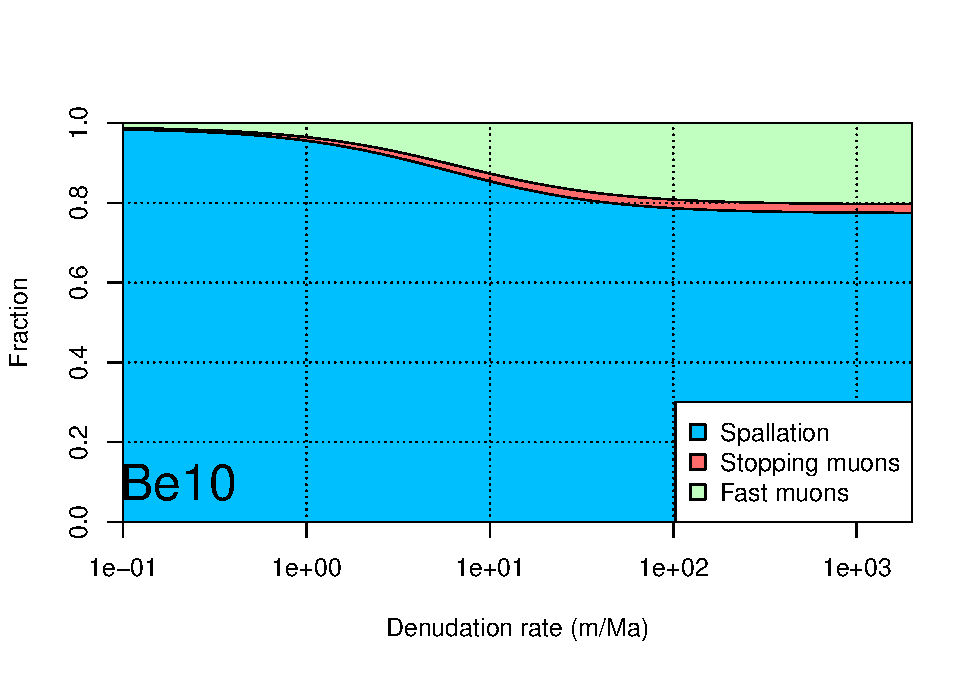
\includegraphics{_main_files/figure-latex/unnamed-chunk-30-1.pdf}

\hypertarget{refs}{}
\begin{CSLReferences}{1}{0}
\leavevmode\vadjust pre{\hypertarget{ref-balco2017production}{}}%
Balco, Greg. 2017. {``Production Rate Calculations for Cosmic-Ray-Muon-Produced {10Be} and {26Al} Benchmarked Against Geological Calibration Data.''} \emph{Quaternary Geochronology} 39: 150--73. \url{https://doi.org/gjq4hn}.

\leavevmode\vadjust pre{\hypertarget{ref-balco2008complete}{}}%
Balco, Greg, John O. Stone, Nathaniel a. Lifton, and Tibor J. Dunai. 2008. {``A Complete and Easily Accessible Means of Calculating Surface Exposure Ages or Erosion Rates from {10Be} and {26Al} Measurements.''} \emph{Quaternary Geochronology} 3 (3): 174--95. \url{https://doi.org/fqdvm9}.

\leavevmode\vadjust pre{\hypertarget{ref-borchers2016geological}{}}%
Borchers, Brian, Shasta Marrero, Greg Balco, Marc Caffee, Brent Goehring, Nathaniel Lifton, Kunihiko Nishiizumi, Fred Phillips, Joerg Schaefer, and John Stone. 2016. {``Geological Calibration of Spallation Production Rates in the {CRONUS-Earth} Project.''} \emph{Quaternary Geochronology} 31: 188--98. \url{https://doi.org/f75rvk}.

\leavevmode\vadjust pre{\hypertarget{ref-gosse2001terrestrial}{}}%
Gosse, John C., and Fred M. Phillips. 2001. {``Terrestrial in Situ Cosmogenic Nuclides: Theory and Application.''} \emph{Quaternary Science Reviews} 20 (14): 1475--1560. \url{https://doi.org/cz26h5}.

\leavevmode\vadjust pre{\hypertarget{ref-lifton2014scaling}{}}%
Lifton, Nathaniel, Tatsuhiko Sato, and Tibor J. Dunai. 2014. {``Scaling in Situ Cosmogenic Nuclide Production Rates Using Analytical Approximations to Atmospheric Cosmic-Ray Fluxes.''} \emph{Earth and Planetary Science Letters} 386: 149--60. \url{https://doi.org/f5r46p}.

\leavevmode\vadjust pre{\hypertarget{ref-marrero2016cronusearth}{}}%
Marrero, Shasta M., Fred M. Phillips, Marc W. Caffee, and John C. Gosse. 2016. {``{CRONUS-Earth} Cosmogenic {36Cl} Calibration.''} \emph{Quaternary Geochronology} 31: 199--219. \url{https://doi.org/f75rpt}.

\leavevmode\vadjust pre{\hypertarget{ref-martin2017crep}{}}%
Martin, L. C. P., P.-H. Blard, G. Balco, J. Lavé, R. Delunel, N. Lifton, and V. Laurent. 2017. {``The {CREp} Program and the {ICE-D} Production Rate Calibration Database: {A} Fully Parameterizable and Updated Online Tool to Compute Cosmic-Ray Exposure Ages.''} \emph{Quaternary Geochronology} 38 (March): 25--49. \url{https://doi.org/f92pbm}.

\leavevmode\vadjust pre{\hypertarget{ref-protin2019climatic}{}}%
Protin, Marie, Irene Schimmelpfennig, Jean-Louis Mugnier, Ludovic Ravanel, Melaine Le Roy, Philip Deline, Vincent Favier, et al. 2019. {``Climatic Reconstruction for the {Younger Dryas}/{Early Holocene} Transition and the {Little Ice Age} Based on Paleo-Extents of {Argentière} Glacier ({French Alps}).''} \emph{Quaternary Science Reviews} 221 (October): 105863. \url{https://doi.org/gjq4nd}.

\leavevmode\vadjust pre{\hypertarget{ref-stone2000air}{}}%
Stone, John O. 2000. {``Air Pressure and Cosmogenic Isotope Production.''} \emph{Journal of Geophysical Research: Solid Earth} 105 (B10): 23753--59. \url{https://doi.org/fbsd87}.

\leavevmode\vadjust pre{\hypertarget{ref-uppala2005era40}{}}%
Uppala, S. M., P. W. KÅllberg, Adrian J. Simmons, U. Andrae, V. Da Costa Bechtold, M. Fiorino, J. K. Gibson, et al. 2005. {``The {ERA-40} Re-Analysis.''} \emph{Quarterly Journal of the Royal Meteorological Society} 131 (612): 2961--3012. \url{https://doi.org/fthgs7}.

\end{CSLReferences}

\end{document}
